\section{Overview of our proposed probabilistic models for harmonization}

%%%%%%%%%%%%%%%%%%%%%%%%%%%%%%%%%%%%%%%%%%%%%%%%%%%%%%
\subsection{Joint modeling of scRNA-seq datasets}
%%%%%%%%%%%%%%%%%%%%%%%%%%%%%%%%%%%%%%%%%%%%%%%%%%%%%%
We consider a collection of scRNA-seq datasets (Figure~\ref{scanviscanvi_presentation}ab). After using a standard heuristic to filter the genes and generate a common (possibly large) gene set of size $G$, we obtain a concatenated dataset that may be represented as a matrix. Individual entries $x_{ng}$ of this matrix measures the expression of gene $g$ in cell $n$. Additionally, we use the integer $s_n$ to denote the dataset of origin for each cell $n$. Finally, a subset of the cells may be associated with a cell state annotation $c_n$, which can describe either discrete cell types or hierarchical cell types. More complex structures over labels such as gradients are left as a future research direction. 

Since the problem of data harmonization of single-cell transcriptomics is difficult and can potentially lead to over-correction~\cite{batchfalsede}, we propose a fully-generative method as a robust and principled approach to address it. In our previous work~\cite{scvi}, we built single-cell Variational Inference (scVI), a deep generative model where the expression level $x_{ng}$ is zero-inflated negative binomial (ZINB) when conditioned on the dataset identifier ($s_n$), and two additional latent random variables. The first, which we denote by $l_n$, is a one-dimensional random variable accounting for the variation in capture efficiency and sequencing depth. In practice, we noticed that this random variable is highly correlated to the library size~\cite{scvi}. The second, which we denote as $z_n$, is a low dimensional random vector that represents the remaining variability~(Figure~\ref{scanviscanvi_presentation}b). This vector is expected to reflect biological differences between cells, and can be effectively used for visualization, clustering, pseudotime inference and other tasks. Since the scVI model explicitly conditions on the dataset identifier (in the sense that it learns a conditional distribution), it provides an effective way of controlling for technical sample-to-sample variability. However, scVI is unsupervised and does not make use of the available annotations $c_n$, which can further guide the inference of an informative latent representation $z_n$. To this end, we present a more refined hierarchical structure for $z_n$. We draw $z_n$ as a mixture conditioned on the cell annotation $c_n$ and another latent variable $u_n$, accounting for further biological variability within a cell type. We name the resulting approach single-cell ANnotation using Variational Inference (scANVI). 

The variables $z_n$, inferred either with scVI or scANVI, provide an embedding of all cells in a single, joint latent space. Since this latent space is inferred while controlling for the dataset of origin ($s_n$), it inherently provides a way to address the harmonization problem. The annotation of unlabeled cells can therefore be conducted with scVI using their proximity to annotated cells in the joint latent space (e.g., using majority vote over the $k$-nearest neighbors). The scANVI model provides a more principled way to annotate cells, namely through a Bayesian semi-supervised approach. Once fitted, the model is able to provide posterior estimates for the unobserved cell state $c_n$, which can be particularly useful when labels cannot be entirely trusted. 


\begin{figure}
\centering
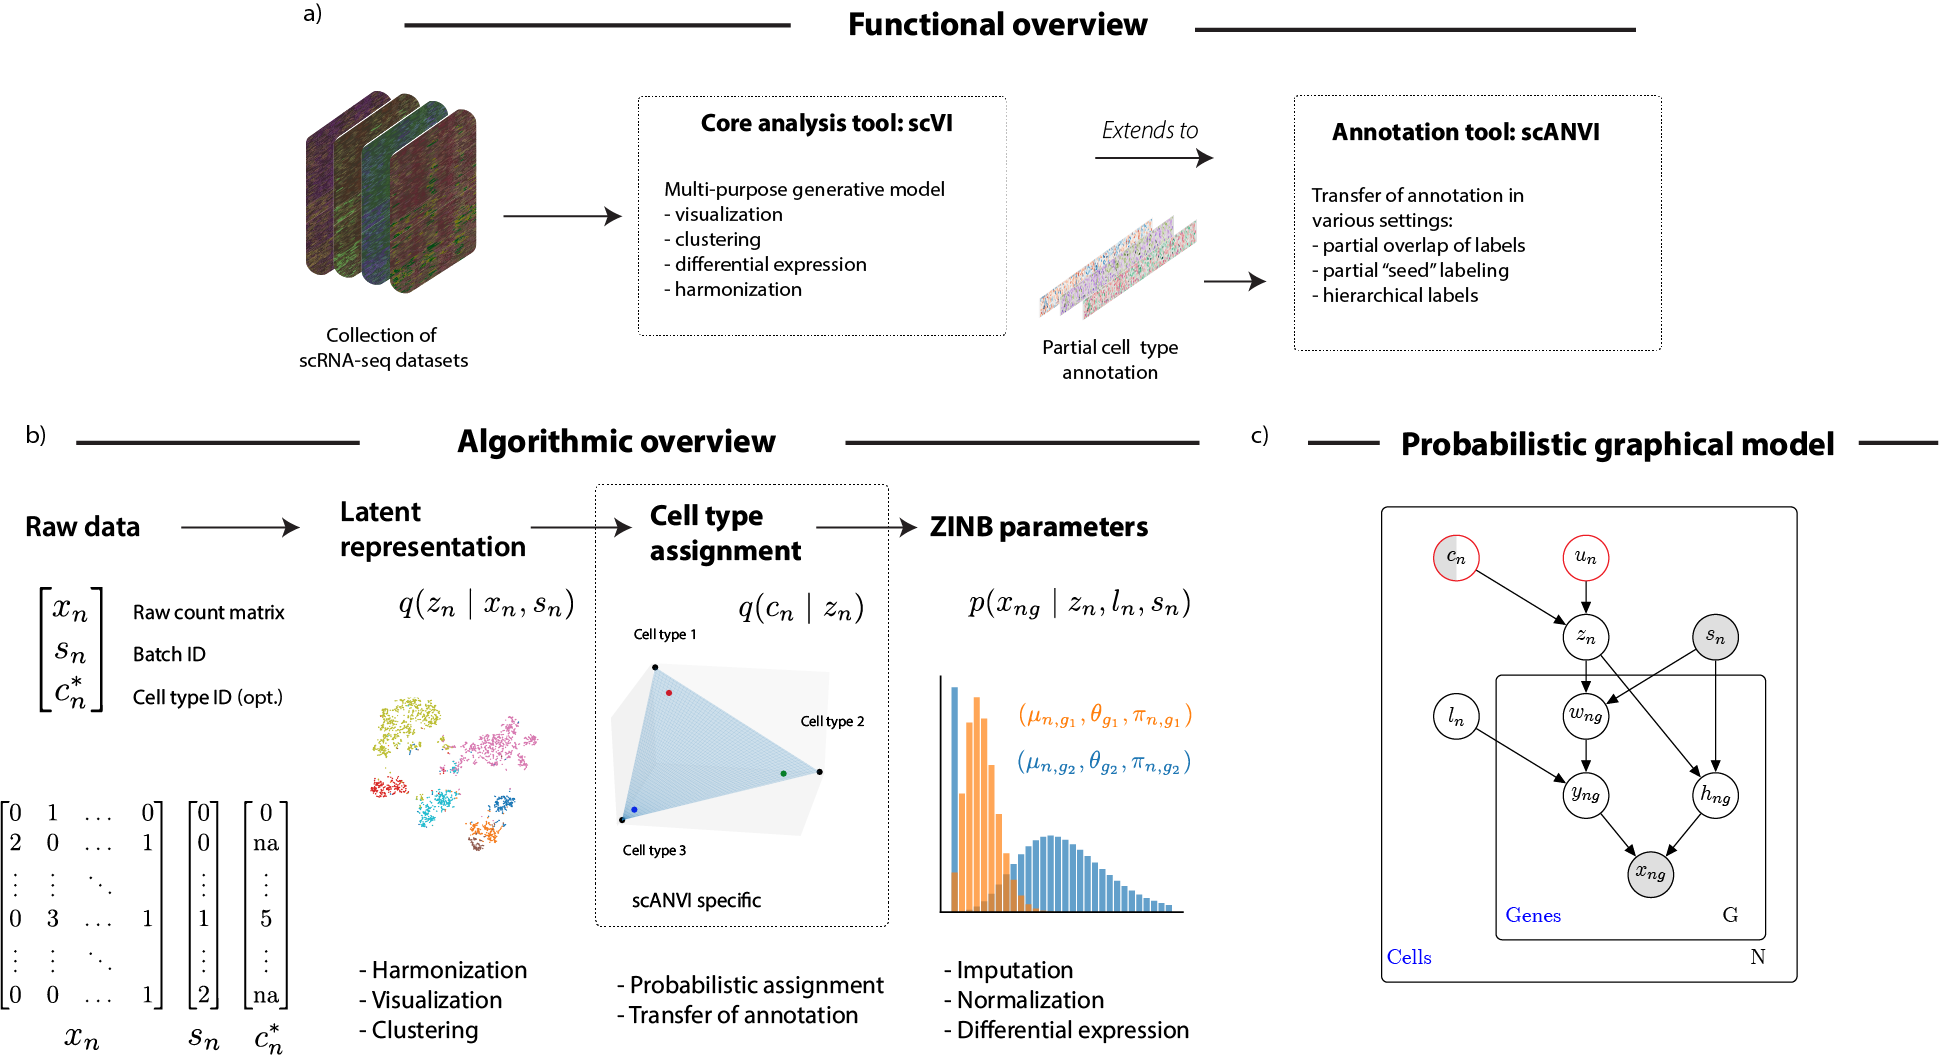
\includegraphics[width=\textwidth]{figures/Figure1.png}
\caption[Harmonization and annotation of scRNA-seq datasets with generative models]{Harmonization and annotation of scRNA-seq datasets with generative models. $(a)$ Functional overview of the methods proposed in this chapter. $(b)$ Schematic diagram of the variational inference procedure in both of the scVI and scANVI models. We show the order in which random variables in the generative model are sampled and how these variables can be used to derive biological insights. $(c)$ The graphical models of scVI and scANVI. Vertices with black edges represent variables in both scVI and scANVI, and vertices with red edges are unique to scANVI. Shaded vertices represent observed random variables. Semi-shaded vertices represent variables that can be either observed or random. Empty vertices represent latent random variables. Edges signify conditional dependency. Rectangles (``plates'') represent independent replication.}.
\label{scanviscanvi_presentation}
\end{figure}


\subsection{Definition of the generative model for scANVI}

In our generative model, we assume each cell $n$ is an independent realization of the following generative process. Let $K$ be the number of datasets and $C$ be the number of cell types across all datasets (including cell types that are not observed). Let $\mathbf{c}$ describe the expected proportion of cells for each cell type. As in general this information is not available to the user, we consistently use a non-informative prior $\mathbf{c} = \nicefrac{1}{C}$ in the chapter. Although some prior information about proportions of cell type is generally accessible, we observe that using the non-informative prior allows us to recover the correct proportion of cells. In addition, in comparative studies such as disease case-control comparisons, or between tissue comparisons of immune cells \cite{schafflick2019ms} we might not want to bias the estimate of cell-type proportion by prior knowledge. All in all, adjustment of the prior $\mathbf{c}$ is not required.  Latent variable 
\begin{align}
c_n \sim  \mathrm{Multinomial}(\mathbf{c}),
\end{align}
describes the cell type of the cell $n$. Latent variable  
\begin{align}
    u_n \sim \mathcal N(0, I),
\end{align}
is a low-dimensional random vector describing cell $n$ within its cell type. Conceptually, this random variable could describe cell-cycles or sub-cell types. By combining cell type information $c_n$ and random vector $u_n$, we create a new low-dimensional vector
\begin{align}
    z_n  \sim \mathcal{N}(f^{\mu}_{z} (u_n, c_n), f^{\sigma}_{z} (u_n, c_n)),
\end{align}
where $f^{\mu}_{z}$ and $f^{\sigma}_{z}$ are two functions parametrized by neural networks. Let $s_n$ encode the dataset information. Given $l_\mu \in \mathbb{R}_+^K$ and $l_\nu \in \mathbb{R}_+^K$ specified per dataset as in~\cite{scvi}, latent variable
\begin{align}
    l_n \sim \textrm{LogNormal}(l^{s_n}_\mu, l^{s_n}_\nu),
\end{align} 
encodes a cell-specific scaling factor. As the prior are adjusted per dataset, our inference procedure will shrink the posteriors towards dataset specific values. This is particularly useful when aligning datasets with dramatically different library size values. Let $\theta \in \mathbb{R}_+^G$ encode a gene specific inverse dispersion parameter (inferred as in~\cite{scvi}). Conditional distribution $x_{ng} \mid z_n, l_n, c_n, s_n$ is conform to the one from the scVI model
\begin{align}
w_{ng} &\sim \mathrm{Gamma}(f^g_w(z_n, s_n), \theta_g)\\
y_{ng} &\sim \mathrm{Poisson}(l_nw_{ng})\\
h_{ng} &\sim \mathrm{Bernoulli}(f^g_h(z_n, s_n))\\
x_{ng} &=
\begin{cases}
y_{ng} & \text{ if } h_{ng} = 0\\
0 & \text{ otherwise}\\
\end{cases},
\end{align}

where $f_w$ and $f_h$ are functions parametrized by neural networks. $f_w$ has a final softmax layer to represent normalized expected frequencies of gene expression as in~\cite{scvi}. Let us note that the resulting distribution for the counts is zero-inflated negative binomial. However, it is straightforward using our implementation to use a negative binomial or a Poisson noise model instead. In this model, annotation $c_n$ can be either observed or unobserved following~\cite{VFAE, m1m2}, which is useful in our applications where some datasets would come partially labeled or unlabeled. Only the first part of the generative model, as separated above, differs from the original scVI formulation. This corresponds to the top part of the new representation of the graphical model in Figure~\ref{scanviscanvi_presentation}b. 



\subsection{Variational inference recipe}

We rely on collapsed variational inference, a standard approximate Bayesian inference procedure that consists in analytically integrating over some of the random variables~\cite{NIPS2006_3113} before optimizing the parameters. As we proved in~\cite{scvi}, we can integrate the random variables $\{ w_{ng}, y_{ng}, h_{ng} \}$ to simplify our model at the price of a looser though tractable lower bound ($x_{ng} \mid z_n, l_n, s_n$ is zero-inflated negative binomial). This procedure reduces the number of latent variable and avoids the need for estimating discrete random variables, which is a harder problem. We then use variational inference, neural networks and the stochastic gradients variational Bayes estimator~\cite{aevb} to perform efficient approximate inference over the latent variable $\{ z_n, u_n, c_n, l_n\}$. We assume our variational distribution factorizes as:
\begin{align}
q_\Phi(c_n, z_n, l_n, u_n \mid x_n, s_n) = q_\Phi(z_n \mid x_n)q_\Phi(c_n \mid z_n)q_\Phi(l_n \mid x_n)q_\Phi(u_n \mid c_n, z_n).
\end{align}

Following~\cite{VFAE, m1m2}, we derive two variational lower bounds: one $\mathcal{L}$ in the case of $c_n$ observed for $p_\Theta(x_n, c_n \mid s_n)$ and a second $\mathcal{U}$ in the case of $c_n$ non-observed for $p_\Theta(x_n \mid s_n)$ where $\Theta$ are all the parameters (neural networks and inverse-dispersion parameters). 

We derive the \emph{evidence lower bound} (ELBO) and detail the training details in the following notes. Briefly, we optimize the sum $\text{ELBO} = \mathcal{L} + \mathcal{U}$ over the neural networks parameters and the inverse-dispersion parameters (in a variational Bayesian inference fashion). Remarkably, the approximate posterior $q_\Phi(c_n \mid z_n)$ can be used as a classifier, assigning cells to cell types based on the location on the latent space. 

We sample from the variational posterior using the reparametrization trick~\cite{aevb} as well as ``mini-batches'' from the dataset to compute unbiased estimate of the objective gradients' with respect to the parameters. We use Adam~\cite{adam} as a first-order stochastic optimizer to update the model parameters. 

\subsubsection{Evidence Lower Bound decomposition}
We drop the parameters $\Theta$ (resp. $\Phi$) of the generative model (resp. the variational distribution) for notational convenience, as well as the conditioning on the batch identifier $s$. We report the evidence lower bound (ELBO) only for one sample (i.e one cell) and drop the index notations by substituting $\{x_n, z_n, u_n, c_n, l_n\}$ by $\{x, z, u, c, l\}$. This is without loss of generality since all the cells are independent and identically distributed under our model.

We derive the ELBO in the case where $c$ is not observed (almost same calculations resolve the case where $c$ is observed). Similar derivations can be found in the variational autoencoder literature~(e.g, \cite{m1m2}). We assume our variational distribution factorizes as:
\begin{align}
    q(c, z, u, l \mid x) = q(z \mid x)q(c \mid z)q(u \mid z, c)q(l \mid x).
\end{align}
In this case, we may simply apply Jensen's inequality weighted by the variational distribution~$q(z, u, l, c \mid x)$:
\begin{align}
    \log p(x) &\geq \Elog{\qall}{\frac{p(x, z, u, c, l)}{\qall}} \\
    &= \Elog{\qall}{\frac{p(x \given z, l)p(z \given u, c)p(c)p(u)p(l)}{\qall}}.
\end{align}
Then, by decomposing this last term, we obtain the following lower bound:
\begin{align}
\begin{split}
    \log p(x) & \geq \underbrace{\Elog{\qall}{p(x \given z, l)}}_{\text{\emph{(i)}}} + \underbrace{\Elog{\qall}{\frac{p(z \given u, c)}{q(z \given x)}}}_{\text{\emph{(ii)}}} \\
    & \qquad + \underbrace{\Elog{\qall}{\frac{p(c)}{q(c \given z)}}}_{\text{\emph{(iii)}}}+ \underbrace{\Elog{\qall}{\frac{p(u)}{q(u \given z,c)}}}_{\text{\emph{(iv)}}} \\
    & \qquad + \underbrace{\Elog{\qall}{\frac{p(l)}{q(l \given x)}}}_{\text{\emph{(v)}}}
\end{split}
\label{scanvielbo}
\end{align}
Then we simplify each individual term of the ELBO in \ref{scanvielbo} by recognizing KL divergence terms. In particular, we use subscript notation $\KLG{.}{.}$, and $\KLM{.}{.}$ to denote Gaussian and multinomial KL divergences.
\begin{align}
    \Elog{\qall}{p(x \given z, l)} &= \Elog{q(z \given x)q(l \given x)}{p(x \given z, l)} \tag{i}\\
    \Elog{\qall}{\frac{p(z \given u, c)}{q(z \given x)}} &= \E{q(z \given x)}{\Elog{q(u \given z,c)q(c \given z)}{\frac{p(z \given u, c)}{q(z \given x)}}} \tag{ii}\\
&= \E{q(z\given x)}{\sum_{c=1}^K q(c \given z) \Elog{q(u \given z,c)}{\frac{p(z \given u, c)}{q(z \given x)}}} \notag \\
    \Elog{\qall}{\frac{p(c)}{q(c \given z)}} &= \E{q(z \given x)}{ \underbrace{\sum_{c=1}^K q(c \given z) \log \frac{p(c)}{q(c \given z)}}_{-\KLM{q(c \given z)}{p(c)}} } \tag{iii}\\
    \Elog{\qall}{\frac{p(u)}{q(u \given z,c)}} &= \E{q(z \given x)}{ \sum_{c=1}^K q(c \given z) \underbrace{\Elog{q(u \given z, c)}{ \frac{p(u)}{q(u \given z, c)}}}_{-\KLG{q(u \given z, c)}{p(u)}} } \tag{iv}\\
    \Elog{\qall}{\frac{p(l)}{q(l \given x)}} &= -\KLG{q(l \given x)}{p(l)}  \tag{v}
\end{align} 


\subsection{Customized training procedures}
In order to train scANVI properly, several options are possible to train all the parameters ($\theta$ from the generative model, $\phi$ from the variational distribution except the labels' posterior and $\phi^{\mathcal{C}}$ from the labels' posterior exclusively). In all cases, parameters $\theta$ and $\phi$ should minimize the evidence lower bound 
\begin{align}
    \mathcal{J} = \mathcal{L} + \mathcal{U},
\end{align}
decomposed over the labeled samples $\mathcal{L}$ and unlabeled samples $\mathcal{U}$. Furthermore,~\cite{m1m2} suggests to jointly optimize a modified objective that penalize the ELBO by a classification loss $\mathcal{C}$ on the labeled data so that the parameters $\phi^{\mathcal{C}}$ also benefits from the learned data. They introduce the modified objective function 
\begin{align}
\mathcal{J}_{\alpha} = \mathcal{J} + \alpha \cdot \mathcal{C},
\end{align}
where $\alpha$ is a parameter set by cross-validation. This modified lower bound can be interpreted as placing a Dirac prior on $c$~\cite{m1m2} or as a correction term for noisy labels~\cite{noisylabels}. In their procedure, $\mathcal{J}_\alpha$ is optimized with respect to all parameters $[\theta, \phi, \phi^{\mathcal{C}}]$ and for a fixed number of epochs. This joint training procedure is appealing as it shapes the latent space directly, through the modification of the encoder’s weights. However, we found this approach to have two limitations. First, this joint training breaks down the mixing in the latent space in the case of transferring labels from one dataset to another. We attribute this to the loss $\mathcal{C}$ having only contributions from a unique dataset. Second, we did not find convenient to choose the optimal value for the parameter $\alpha$ and concluded it may not be desirable for a practitioner either. 

We use in scANVI an alternate training procedure which deletes the need for $\alpha$ and has better performance in the setting of transferring annotations. We aggressively train the classifier separately, updating the parameters $\phi^\mathcal{C}$ for $c > 1$ epochs for every single epoch of updating $[\theta, \phi]$. The total number of epochs is fixed and chosen high enough to guarantee convergence. In the case of a single dataset (resp. transfer of labels), we use $c=1$ (resp. $c=100$) epochs of classifier training in between each variational update. This helps the classifier correctly identify cell types at the end of each epoch of updating $\phi^\mathcal{C}$. This is a clearly advantageous procedure, because it then improve indirectly the latent space quality, through the next steps of optimization. 




\subsection{Choice of hyperparameters}

Notably, scANVI and scVI both have a certain number of hyperparameters. In the following evaluations, conducted on different datasets and different scenarios, we use the exact same set of hyperparameters in order to demonstrate that our methods can be applied with a minimal requirement of hyperparameter tuning. 

For all harmonization tasks in this chapter, we consistently use the same set of hyperparameters. Each network has exactly 2 fully-connected layers, with 128 nodes each. The number of latent dimensions is 10, the same as other algorithms for benchmarking purposes (e.g., the number of canonical correlation vectors used in Seurat Alignment). The activation functions between two hidden layers are all ReLU. We use a standard link function to parametrize the distribution parameters (exponential, logarithmic or softmax). Weights for the first hidden layer are shared between $f_w$ and $f_h$. We use Adam with $\eta = 0.001$ and $\epsilon = 0.01$. We use deterministic warmup~\cite{warmup} and batch normalization~\cite{batchnorm} in order to learn an expressive model. When we train scANVI, we therefore assume that the data come from a set of $C_\text{observed}+C_\text{unobserved}$ populations, each generated by a different distribution of $z_n$ values. This set includes the $C_\text{observed}$ populations for which annotated cells are available, and $C_\text{unobserved}$ population that accounts for cell types for which an annotation is not available to the algorithm. 

We also provide a robustness study for hyperparameters in the context of harmonization in Figure~\ref{scanvirobustness_supplement}. 

\subsection{Alternative model choices}

\subsubsection{Zero-inflation in the context of harmonization}
 In this chapter, we mainly rely on a zero-inflated negative binomial (ZINB) distribution for the counts --- which is a widely used model for single cell transcriptomics data. Recent research however suggests that for some technologies such as droplet-based UMI single-cell protocols, the abundance of zero mainly may be explained only by limited sensitivity and subsampling effect \cite{svensson2019droplet}. On the other hand, zero-inflated might be a realistic addition to count distributions for describing full-length plate-based technologies data \cite{vieth2017powsimr}. Indeed, it has been hypothesized that PCR duplication or uneven fragment sampling may be responsible for zero-inflation in plate-based technologies \cite{svensson2019droplet}. Still, no definite conclusion can be drawn about which distribution better fits UMI technologies or full-length method. Although full-length methods seem more affected by technical noise, they also provide extra information at the transcript resolution that is lost in droplet-based UMI methods. Consequenly, many consortia have chosen to obtain data by both full-length and UMI methods~\cite{quake2018single,ecker2017brain}. A method that can flexibly use different distribution and appropriately these two data types is therefore extremely valuable for analyzing collections of single cell transcriptomics data. 
 
 scVI and scANVI are both flexible to use both ZINB and NB methods and we show in Figure~\ref{scanviZINB_NB} that the benchmarking results are similar using both methods in all four datasets used in our benchmarking procedure. However, we observed that for MarrowTM dataset, using the ZINB version of scVI does perform better in terms of harmonization. Since in this case, we are merging a 10x dataset with a Smart-Seq2 dataset, we compared the average zero-inflation parameter for each gene in each dataset and found that the differences between Smart-Seq2 and 10x are significantly skewed to the right (more zero-inflation in Smart-Seq2, $p$=6.3e-31, using a D'Agostino-Pearson $K^2$ test). Finally, we also performed differential expression with negative binomial versions of scVI and scANVI and show that results are similar (Figure~\ref{scanviDE_NB}). These results show that both NB and ZINB model can be used in scVI and scANVI and in most instances, downstream analysis might not be impacted by this modeling choice. Interestingly, our model successfully learns the difference in the degree of zero-inflation in different datasets while merging them and exploits this information when necessary.
 
 
 \subsubsection{Library-size prior for scVI and scANVI}
 Besides zero-inflation, another major difference between sequencing technologies is the sequencing depth. scVI and scANVI both make use of technical scalar factors that have a batch-specific prior, and are therefore extremely suited for this setting. 
 To evaluate the effectiveness of both the model and the prior choice, we compute the negative log likelihood of the scVI model using ZINB with batch-specific library size prior, ZINB with shared library size prior, NB with a batch-specific library size prior, and NB with shared library size prior. All four models are fit on two pairs of datasets, DentateGyrus (Fluidigm C1 and 10x) and MarrowTM (10x and SmartSeq2). Since only the second pair is a comparison between UMI and full-length datasets, we expect the differences between the four model choices to be larger in the MarrowTM comparison, and that ZINB with batch-specific library size prior to have the highest likelihood (reported in Table~\ref{library_size_ll}). 

\begin{table}
\centering
\begin{small}
\begin{tabular}{lcc}
    \toprule
\textbf{Negative log-likelihood}           & \textbf{DentateGyrus} & \textbf{MarrowTM} \\
\midrule
\textbf{ZINB model / batch-specific prior}                        & 514.5        & 2339.8   \\
\textbf{ZINB model / shared prior}  & 513.8        & 2349.2   \\
\textbf{NB model / batch-specific prior}                         & 523.4        & 2531.3   \\
\textbf{NB model / shared prior}   & 524.0        & 2544.1  \\
\bottomrule
\end{tabular}
\end{small}
\caption{ The effect of library size prior and count distribution on the model likelihood
}

\label{library_size_ll}
\centering
\end{table}


\subsection{Related machine learning literature}
Our approach relates to the machine learning literature in two major aspects. First, we relate the problems of harmonization and annotation to the litterature of domain adaptation or covariate shift. Second, we present all the different options for performing semi-supervised learning with variational autoencoders (VAEs) and further explain how they relate to scANVI.

\subsubsection{Domain adaptation}
In the supervised learning framework, data is drawn from a distribution $\mathbb{P}_X$ and one posits a conditional distribution $\mathbb{P}_{Y \mid X}$ from which to draw the labels. There are multiple flavors of domain adaptations~\cite{kouw2019review}. We focus here in the setting where one observes paired data on a certain source domain $\mathbb{P}_X^{S}\mathbb{P}_{Y \mid X}$ but no labels on a target domain $\mathbb{P}_X^{T}$ with $\mathbb{P}_X^{S} \neq \mathbb{P}_X^{T}$ (commonly referred to as distribution shift, or \textit{covariate shift} in the statistical literature). Our problem of single-cell annotation is much related to this variant of supervised domain adaptation where one observes the cell labels for one dataset and wishes to transfer it to another (annotated) dataset. This is a well-established research area in computer vision, where algorithms such as NBNN~\cite{6751221} and JDA~\cite{6751384} are used to transfer labels over datasets of images (e.g., with different lightning conditions, collections of images). As these algorithms might not scale to millions of samples, a notable contribution is the 
DANN framework~\cite{ganin2016domain} which learns a adversarial classifier to in order to generalize to the new (unlabelled) dataset. This approach is justified from the statistical theory perspective as the adversarial regularization is equivalent to controlling for the $\mathcal{H}$-divergence between source domain $\mathbb{P}_X^{S}$ and target domain $\mathbb{P}_X^{T}$. Another notable contribution is the variational fair autoencoder, which focuses on semi-supervised domain adaptation with VAEs~\cite{VFAE} by adding a maximum mean discrepency \cite{MMD} loss between source and target latent distributions. 

Moving away from the supervised domain adaptation scenario, recent work based on generative adversarial networks~\cite{goodfellow2014generative} focuses on unsupervised domain adaptation of \emph{unpaired} datapoints. This problem is relevant to the scRNA-seq methodology since one never gets to observe the same cell several times (the protocol is a destructive process). CycleGAN~\cite{zhu2017unpaired} is based on the idea of cycle consistency (a translator that would transform a french sentence into english and then back to french again should be the identity map). This idea was then improved by Cycada~\cite{pmlr-v80-hoffman18a}, which adds more consistency to the objective function. StarGAN~\cite{choi2018stargan} extended CycleGAN to multiple domains while reducing the overall complexity. Finally, MAGAN~\cite{amodio2018magan} proposed to add a correspondence loss to further orient the manifold alignment and facilitate the inference. Notably, MAGAN~\cite{amodio2018magan} was also applied to merging scRNA-seq and CyTOF data.

\subsubsection{Semi-supervised learning with variational autoencoders}
Extending scVI to semi-supervised learning took some design that we describe here. Our first attempt was based on the M2 model~\cite{m1m2}. While this algorithm performed a posteriori as good or better than the final version of scANVI (in terms of cross-validation estimate of the cell type prediction accuracy), it restrained our latent space $z$ to be conditioned on the cell type label (as in the conditional VAE~\cite{NIPS2015_5775}) and it was not possible anymore to visualize the latent space, which is an crucial practice in scRNA-seq data analysis~\cite{Becht2018}. We therefore turned to extending scVI based on the M1 + M2 model \cite{m1m2}, which enabled both a flexible modeling of cell types and visualization of a joint latent space for all cells. We also tried more complicated models based on the M1 + M2 model such as ADGM~\cite{maaloe2016auxiliary} and LVAE~\cite{rasmus2015semi} but did not find them to contribute significantly enough to the accuracy, which might be either due to the labeling errors in the dataset, because dividing cells into cell types is a relatively easy problem in most regimes (e.g., not considering rare cell types) or because of the limited sample size in the datasets we consider. 


\subsection{Related scRNA-seq harmonization work}
\label{scanviassumptions}

\subsubsection{Why is harmonization a subtle problem?}
Harmonization is a hard and ill-defined problem. Especially, it can be difficult to formulate exactly its objective and at which level of granularity the ``harmonization'' is expected. Let us take the example of two scRNA-seq datasets of peripheral blood mononuclear cells. If we assume that these datasets that are exact biological replicates and with the same experimental conditions, then the problem is well defined. We wish to identify latent variables that govern these biological processes (for example, clear demarcation of cell types). Fundamentally, this is possible because we made a  non-confounder assumption, and therefore, removing in a principled way all the variation in the data that corresponds to batches is reasonable. 

However, if we consider a more complex although also more common case, the biology might be slightly different from one dataset to another. For example, in the case of T cell activation (one stimulated sample and one control sample), we expect that the overall clusters should stay similar. At a broader level, CD4 T cells should cluster together, as for all the other cell types. However, a non-negligible proportion of T cells will express markers of activation. In this case, forcing the latent spaces to exactly overlay might be problematic in the sense that this subtle signal of activation will be lost. One might think about the activation signal as a confounding factor for harmonization, and this makes the overall problem much more difficult (ill-posed).

Therefore, it is extremely important to state how different models perform harmonization and what are their underlying hypotheses and modeling capabilities.

\subsubsection{State-of-the-art approaches}

scmap~\cite{scmap} proposes a new gene filtering method to select gene that are claimed to be invariant to batch-effects. However, it is clear that over filtering can lead to ignoring biological information.  
MNN~\cite{MNN} assumes that the topology of cell types can be easily resolved by a $k$-nearest neighbors graph, where neighborhoods are defined with respect to the cosine distance. This allows MNN~\cite{MNN} and all the neighbor-matching-based approaches~\cite{SEURAT3,scanorama} to remarkably merge batches with the risk of also merging cell types in the case where they are not detectable with this normalization scheme. 
SAUCIE~\cite{saucie} and MMD ResNet~\cite{resnetbatcheffect} both propose to perform batch-correction by adding on their objective function a non-parametric measure of distance between distributions (maximum mean discrepancy). This approach specifically assumes that each dataset has the same cell type composition and the same biological signal. Therefore, SAUCIE and ResNet are susceptible to perform over-correction. 
Seurat Alignment~\cite{seurat} relies on a milder assumption that there is a common signal exactly reproducible between the two datasets and that CCA capture most of the biological variation. This is not obviously true considering limited suitability of linear Gaussian model for scRNA-seq. 
Seurat anchors~\cite{SEURAT3} relies on CCA and suffers from the same problems as MNN with its specific normalization scheme. 
Finally, the recent LIGER~\cite{LIGER} method at first sight seems like a non-probabilistic version of scVI since it also learns a degenerate conditional distribution via its integrative non-negative matrix factorization~\cite{LIGER} (NMF is a noisy-less version of a Gamma-Poisson generative model). However, it has a further quantile normalization of the latent spaces within clusters. First, the output of the clustering algorithm is not necessarily correct and could perturb downstream analyses. Second, if a cell type would be slightly different from one condition to another, this information would be lost in the final latent space. Overall, all these correction methods can therefore potentially lead to over-correction and statistical artifacts~\cite{batchfalsede}.


\subsubsection{Our approach}
scVI and scANVI perform harmonization by learning a common generative model for a collection of gene expression probability distributions $\left[p(x \mid z, s)\right]_{s \in \{1, \ldots, K\}}$ indexed by the dataset-identifier $s$. The statistical richness of the collection of conditional distributions dictates the flexibility of our model towards integrating datasets. 

Another notable factor that sensibly contributes to harmonization capabilities is the prior for cell-specific scaling factor $l_n$ that is dataset-specific. This helps probabilistically removing library-size caused discrepancies in the measurements and is more principled than normalization of the raw data~\cite{vallejos2017norm}. Another important parameter is the parametrization of the neural network that maps variables $(z, \gamma)$ to the expected frequencies $\mathbb{E}[w \mid z, s] = f_w(z, s)$. Since our function $f_w$ is now potentially non-linear, our model can benefit from more flexibility and fit batch-specific effects locally for each cell types or phenotypical condition. Especially, depending on how one designs the neural architecture of $f_w$, it is possible to more flexibly correct dataset-specific effects. More specifically, we treat $f_w$ as a feed-forward neural network for which at each layer we concatenate the batch-identifier with the hidden activations. A consequence of this design is that with more hidden layers in $f_w$, less parameters are shared and the family of distributions $\left[p(x \mid z, s)\right]_{s \in \{1, \ldots, K\}}$ has more flexibility to fit batch-specific effects (Figure~\ref{scanvirobustness_supplement}a-c). Conversely, when the latent dimension grows, the generative network has less incentive to use the dataset covariate and might mildly duplicate the information in its latent space (Figure~\ref{scanvirobustness_supplement}d-f). Throughout the chapter, we have fixed those parameters and show competitive performance for all our datasets.

Another insight comes from how the variational distribution $q(z \mid x, s)$ is parametrized. Our neural networks play the role of an explicit stochastic mapping from the gene expression $x_n$ of a single-cell $n$ to a location in a latent space $z_n$ (a standard theme in scRNA-seq analysis). With this map, we match an empirical distribution in gene expression space (i.e, a dataset) $p_{\text{data}}(x, s) = \sum_n \delta_{(x_n, s_n)}(x, s)$, with a certain distribution on the latent space $p_{\text{data}}(z) = \sum_n \delta_{\Phi(x_n, s_n)}(z)$. In certain cases, even though we designed this latent space to represent biological signal, the transformed dataset might still be confounded by technical effects~\cite{HCV}. In particular, this effect is susceptible to be severe when the generative model is not flexible enough to fit the dataset-specific effects or has a model misfit (as in, to some extent, the case with the CCA of~\cite{seurat} that assumes the data is log-normal). In this case, the go-to method is to empirically constrain the mapping (i.e the variational network in our case or the latent space itself in the case of Seurat) to match the collections of variables $p_{\text{data}}(z, s)_{s \in \{1, \ldots, K\}}$. This is what is done via all the methods presented above. Therefore, our method might be improved with respect to the entropy of batch mixing by adding some specific penalties to the loss function, but at the price of risking to over-correct. We have preferred to not add any penalties, which is enough for most applications (especially all those in this chapter). 


\section{Results}
In the following we demonstrate that our framework compares favorably to state-of-the-art methods for the problems of harmonization and annotation in terms of accuracy, scalability, and adaptability to various settings. The first part of the chapter focuses on the harmonization problem and covers a range of scenarios, including harmonization of datasets with varying levels of biological overlap, handling cases where the data is governed by a continuous (e.g., pseudotime) rather than discrete (cell types) form of variation, and processing multiple ($> 20$) datasets. While we demonstrate that scVI performs well in these scenarios, we also demonstrate that the latent space learned by scANVI provides a proper harmonized representation of the input datasets --- a property necessary for guaranteeing its performance in the annotation problem. 

In the second part of this result section we turn to the annotation problem and study its two main settings, namely transferring labels between datasets and \textit{ab-inito} labeling. In the first setting we consider the cases of datasets with a complete or partial biological overlap and use both experimentally- and computationally- derived labels to evaluate our performance. In the second setting, we demonstrate how scANVI can be used effectively to annotate a single dataset by propagating high confidence seed labels (i.e., based on marker genes) and by leveraging a hierarchical structure of cell state annotations. Finally, we demonstrate that the generative models inferred by scANVI and scVI can be directly applied for hypotheses testing, using differential expression as a case study. 



%%%%%%%%%%%%%%%%%%%%%%%%%%%%%%%%%%%%%%%%%%%%%%%%%%%%%%
\subsection{Presentation of the datasets}
%%%%%%%%%%%%%%%%%%%%%%%%%%%%%%%%%%%%%%%%%%%%%%%%%%%%%%
We apply our method on datasets generated by a range of technologies (10x Chromium~\cite{zheng2017massively, 10x}, plate-based Smart-Seq2~\cite{picelli2014SS2}, Fluidigm C1 \cite{fluidigmXin2016}, MARS-Seq~\cite{jaitin2014massively}, inDrop~\cite{klein2015droplet} and CEL-Seq2~\cite{celseq2016}), spanning different numbers of cells (from a few thousand to over a hundred thousand cells), and originating from various tissues (mouse bone marrow, human peripheral mononuclear blood cells [PBMCs], human pancreas, mouse brain). Datasets are listed and referenced in Table~\ref{scanvidatasets}.


\paragraph{Gene Selection}
A common practice in data harmonization is to perform gene selection prior to harmonization. This assumption is critical when the number of genes that can be taken into account by the algorithm is small and potentially biological signal could be lost. scVI is however designed for large datasets which do not fall into the high-dimensional statistics data regime~\cite{scvi}. Remarkably, there is no need for crude gene filtering as part of our pipeline and we adopt it as part of this publication only for concerns of fairness in benchmarking. For real datasets, we calculated the dispersion (variance to mean ratio) for all genes using Seurat in each dataset and selected $g = 1,000$ genes with the highest dispersion from each. The performance of scVI is not as affected by gene set and we use the same gene selection scheme as in \cite{seurat} to ensure fairness in our comparison. We then took the union of these gene list as input to Seurat Alignment, MNN and scANVI. One exception is the differential expression study for which we kept the gene set ($g=3,346$) to have it match the bulk reference as in~\cite{scvi}. 

\paragraph{Cell type labeling for the Tabula Muris Dataset} 
For the Tabula Muris dataset, cell types are defined by first reducing the dimensions of the data by principal component analysis and then performing nearest-neighbor-graph-based clustering. The labels for Smart-Seq2 and 10x data are derived independently. All cells in both dataset are labeled, but there is also a possibility that they are mislabelled since the labels are computationally derived. Since cells used in Smart-Seq2 are first FACS sorted into each plate, some cell types might have been lost during the sorting process, resulting in incomplete overlap in cell types between the two datasets.

\paragraph{Normalization of SmartSeq2 data} For the MarrowMT-ss2 dataset, we normalized the read counts per gene by relative transcript length (average transcript lengths of a gene divided by average gene length over all genes), and subsequently took the integer part of the normalized count. This is different from standard normalization procedures in that we do not normalize by cell size because cell size normalization can be performed by scVI. And we only keep the integer part of the counts, due to the distributional assumptions made by scVI. The scVI model can to be extended to fit data with amplification bias, however we have not done so for this chapter and thus have to perform this normalization heuristic. 


\begin{table}
\begin{small}
\begin{tabularx}{\textwidth}{lllXl}
\toprule
\textbf{Dataset Name} & \textbf{Tech.} &\textbf{$n$ cells} &  \textbf{Description} & \textbf{Ref.} \\
\midrule

% \textbf{SIM1} & Simulation & 20,000 & simulated by first generating a single dataset with noise in the UMI mode of SymSim, randomly splitting it into two batches and multiplying each batch by a different small gene specific scaling factor.  & \cite{symsim}\\[0.2cm]

% \textbf{SIM2} & Simulation & 20,000 & simulated by first simulating the true gene count without noise, splitting randomly into to batches and simulating one batch with UMI noise model and nonUMI noise model in SymSim & \cite{symsim}\\[0.2cm]

% \textbf{SIM3} & Simulation & 20,000 & simulated by simulating two batches of cells that share all other parameters except for a batch-specific Extrinsic Variation Factor (EVF) & \cite{symsim}\\[0.2cm]

\textbf{PBMC-8K} & 10x & 8,381 & peripheral blood mononuclear cells (PBMCs) from a healthy donors; labels extracted from \cite{SCONE} & \cite{10x}\\[0.2cm]

\textbf{PBMC-CITE} &10x & 7,667 & PBMCs  obtained from CITE-seq; labels generated manually by inspection of protein marker level on Seurat clusters &\cite{stoeckius2017simultaneous}\\[0.2cm]

\textbf{PBMC-68K} & 10x & 68,579 & fresh PBMCs collected from healthy donor &\cite{zheng2017massively} \\[0.2cm]

\textbf{PBMC-Sorted} &10x &  94,655 & Bead-purified PBMCs collected from the same donor as PBMC68K  & \cite{zheng2017massively}\\[1cm]

\textbf{MarrowTM-10x} &10x &4,112 & Mouse bone marrow cells collected from two female mice & \cite{quake2018single}\\[0.2cm]

\textbf{MarrowTM-ss2} &  Sma.-Seq2 & 5,351 & FACS sorted cells (B cells, T cells, granulocytes and  Kit (+), Sca-1 (+) and Lin (-) hematopoietic stem cells) from 3 male and 2 female mice, & \cite{quake2018single}\\[1cm]

\textbf{Pancreas-InDrop} & inDrop  & 8,569 & Human Pancreas & \cite{pancreasindrop}\\[0.2cm]

\textbf{Pancreas-CELSeq2} & CEL-Seq2 & 2,449 & Human Pancreas & \cite{pancreascelseq}\\[0.2cm]

\textbf{DentateGyrus-10x} & 10x &5,454 & Mouse Dentate Gyrus & \cite{dentategyrus2018}\\[0.2cm]

\textbf{DentateGyrus-C1} & Fluid. C1 & 2,303 & Mouse Dentate Gyrus & \cite{dentategyrus2018}\\[1cm]

\textbf{CORTEX} & 10x & 160,796  & Mouse Nervous System & \cite{zeisel2018}\\[1cm]

\textbf{HEMATO-Tusi} & inDrop & 4,016 & Hematopoeitic Progenitor Mouse Cells & \cite{Tusi2018}\\[0.2cm]

\textbf{HEMATO-Paul} & MARS-seq & 2,730 & Hematopoeitic Progenitor Mouse Cells & \cite{PAUL2015}\\[1cm]

\textbf{SCANORAMA} & Mixture & 105,476 & human cells from 26 diverse scRNA-seq experiments across 9 different technologies & \cite{scanorama}\\
\bottomrule
\end{tabularx}
\caption[List of datasets used in this chapter]{List of datasets used in this chapter. Note that for the PBMC-Sorted 11 cell types were collected according to the paper but only 10 are available from the 10x website~\cite{10x}.\label{scanvidatasets}}
\end{small}

\end{table}
 



%%%%%%%%%%%%%%%%%%%%%%%%%%%%%%%%%%%%%%%%%%%%%%%%%%%%%%
\subsection{Harmonizing pairs of datasets with a discrete population structure}
%%%%%%%%%%%%%%%%%%%%%%%%%%%%%%%%%%%%%%%%%%%%%%%%%%%%%%
We conducted a comparative study of harmonization algorithms on four different instances, each consisting of a pair of datasets. The first pair (PBMC-CITE~\cite{stoeckius2017simultaneous}, PBMC-8K~\cite{10x}) represents the simplest case, in which the two datasets come from very similar biological settings (i.e., PBMCs) and are generated by the same technology (i.e., 10x) but in different labs (i.e., akin to batch correction). A second scenario is that of similar tissue but different technologies, which we expect to be more challenging as each technology comes with its own characteristics and biases~\cite{Ziegenhain2017}. For instance, some methods (10x, CEL-Seq2) profile the end of the transcript and use Unique Molecular Identifier (UMI) to mitigate inflation in counting, whereas others (e.g., most applications of Smart-Seq2) consider the full length of the transcript without controlling for this potential bias. Additionally, some protocols (e.g., Smart-Seq2) tend to have higher sensitivity and capture more genes per cell compared to others. Finally, studies using droplet based protocols tend to produce much larger numbers of cells compared to plate-based methods. We explore three such cases, including a bone marrow 10x and Smart-Seq2 pair from the Tabula Muris project (MarrowTM-10x, MarrowTM-ss2~\cite{quake2018single}), a pancreas inDrop and CEL-Seq2 pair (Pancreas-InDrop, Pancreas-CEL-Seq2~\cite{pancreasindrop}), and a dentate gyrus 10x and Fluidigm C1 pair (DentateGyrus-10x, DentateGyrus-C1~\cite{dentategyrus2018}). 

Successful harmonization should satisfy two somewhat opposing criteria. On the one hand, cells from the different datasets should be well mixed; namely, the set of $k$-nearest neighbors ($k$NN) around any given cell (computed e.g., using euclidean distance in the harmonized latent space) should be balanced across the different datasets. For a fixed value of $k$, this property can be evaluated using the entropy of batch mixing~\cite{MNN}, which is akin to evaluating a simple $k$-nearest neighbors classifier for the batch identifier. Briefly, the entropy of batch mixing is the average negative entropy of cell type proportion of the $k$-nearest-neighbors of each cell in the harmonized latent space. Higher value for this metric indicates that the harmonized latent space shows strong mixing: the neighbors of each cell is composed of cells from different batches. While this property is important, it is not sufficient, since it can be achieved by simply randomizing the data. Therefore, in our evaluation we also consider the extent to which the harmonized data retains the original structure observed with each dataset taken in isolation. Here, we expect that the set of $k$-nearest neighbors of any given cell in its original dataset should remain sufficiently close to that cell after harmonization. We evaluate this property using a measure we call $k$-nearest neighbors purity, computed as the average percent overlap of the $k$-nearest-neighbors of each cell before and after harmonization. This metric takes value between 0 and 1 and higher values indicate better retainment of structure. This criteria is important, but is maximized by a trivial approach of simply concatenating the latent spaces. Of course, this will result in poor performance with respect to our first measure. Our evaluation therefore relies on both types of measures, namely mixing of data sets and retainment of the original structure. Since our results depend on the neighborhood size $k$, we consider a range of values - from a high resolution ($k=10$) to a coarse ($k=500$) view of the data. 


We compare scVI to several methods, including MNN~\cite{MNN}, Seurat Alignment~\cite{seurat}, ComBat~\cite{combat} and principal component analysis (PCA). In addition, and in order to compare our methods to unpaired data integration approaches based on generative adversarial networks ~\cite{zhu2017unpaired}, we also tested  MAGAN~\cite{amodio2018magan}. However, even after manual tuning of the learning rate hyperparameter, the input datasets remain largely unmixed (Figure~\ref{scanvimagan}). This might be due to the fact that MAGAN was not directly applied to harmonize pairs of scRNA-seq datasets and need more tuning to be applicable in that context. For each algorithm and pair of datasets, we report embeddings computed via a Uniform Manifold Approximation and Projection (UMAP)~\cite{umap}~(Figure~\ref{benchmarking_panel}a, Figure~\ref{scanviEasy1}~-~\ref{scanviTech4}) as well as the two evaluation metrics (Figure~\ref{benchmarking_panel}b-c).

Overall, we observed that scVI compares favorably to the other methods in terms of retainment of the original structure (Figure~\ref{benchmarking_panel}a) and performs well in terms of mixing (Figure~\ref{benchmarking_panel}b) for a wide range of neighborhood sizes and across all dataset pairs. The trade-off of these two aspects of harmonization for a fixed $k$ is shown in Figure~\ref{benchmarking_panel}c, and again scVI and scANVI performs favorably and show up on the top right corner of the scatter plot. scANVI performs slightly better than scVI. Furthermore, because the conservation of $k$-nearest neighbors might be more indicative of a local stability of the algorithm and misses the clustering aspect of the data, we also quantified the conservation of cluster assignments. Towards this end, we used the adjusted Rand index to compare the agreement of a $k$-means clustering algorithm, before and after harmonization (Figure~\ref{benchmarking_panel}d). Reassuringly, our positive results for preservation of the output of a clustering algorithm indicates that scVI and scANVI are also stable with regards to more global aspects of the data.

\begin{table}
\centering
\begin{small}
\begin{tabular}{lcccc}
    \toprule
\textbf{Method}   & \textbf{PBMC8KCITE} & \textbf{MarrowTM} & \textbf{Pancreas} & \textbf{DentateGyrus} \\[0.2 cm]
\midrule
\textbf{scVI}     & 0.73395    & 0.74325  & 0.81425 & 0.5418       \\[0.2 cm]
% \textbf{scVI\_nb} & 0.7648     & 0.71035  & \textbf{0.8281}   & \textbf{0.5915}\\ [0.2 cm]
\textbf{scANVI1}  & 0.74465    & 0.7418   & 0.76625  & 0.55875      \\[0.2 cm]
\textbf{scANVI2}  & \textbf{0.8184}    & \textbf{0.77825}  & 0.78815  & 0.54135      \\[0.2 cm]
\textbf{Seurat}   & 0.7351     & 0.72095  & 0.6174   & 0.4149       \\[0.2 cm]
\textbf{MNN}     & 0.7364     & 0.6783   & 0.76205  & 0.4296       \\[0.2 cm]
\textbf{PCA}      & 0.59895    & 0.6089   & 0.5474   & 0.4179 \\
\bottomrule     
\end{tabular}
\end{small}
\caption[Additional metric for retainment of structure via k-means clusters preservation.]{Additional metric for retainment of structure via $k$-means clusters preservation. For scANVI we perform semi-supervision using the cell type label (not $k$-means cluster labels) from only one of the two datasets. Thus we train two separate models SCANVI1 and SCANVI2. To obtain a measure of clustering conservation, we first run $k$-means clustering in the latent space of dataset 1, then in the harmonized latent space using only cells from dataset 1. We compute the adjusted Rand Index of the two clustering results. We then do the same for dataset 2 and the final score is the average for both datasets.} 
\label{scanviclustering_retainment}
\end{table} 


While scANVI was designed for the problem of cell state annotation, we also wanted to evaluate its ability to harmonize datasets, which can be seen as a prerequisite. To evaluate this, we consider each dataset pair twice, each time using labels from one of the datasets (exploiting the semi-supervision framework of scANVI) and leaving the other one unlabeled. Reassuringly, we found that scANVI is capable of effectively harmonizing the datasets, with a similar performance to that of scVI in terms of entropy of batch mixing and retainment of the original structure (Figure~\ref{benchmarking_panel}). We further explore the performance of scANVI in the annotation problem in the subsequent sections.

\begin{figure}[htp]
    \centering
    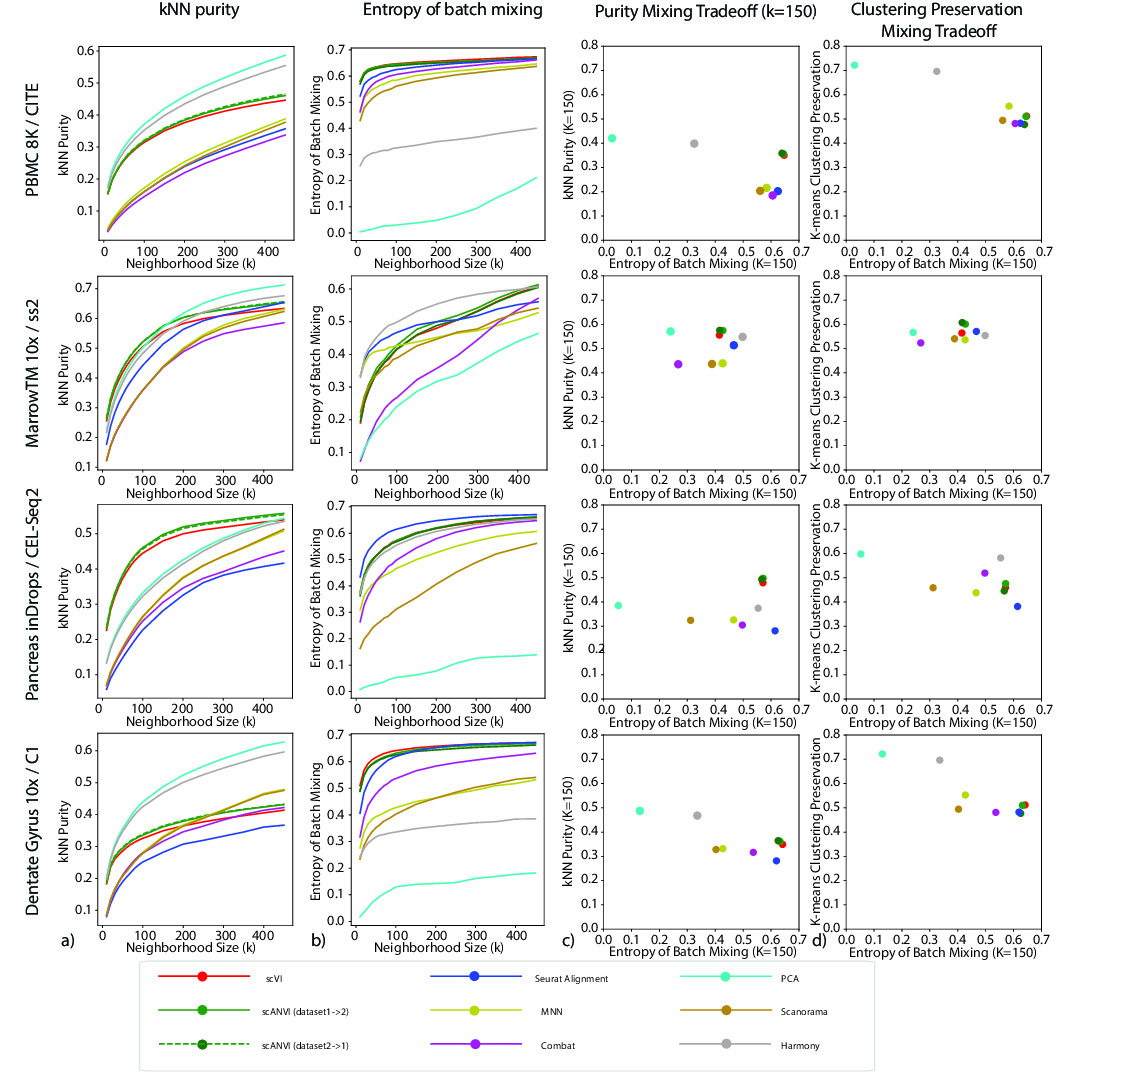
\includegraphics[width=\textwidth]{figures/Fig2.jpeg}
    \caption[Benchmarking of scRNA-seq harmonization algorithms]{Benchmarking of scRNA-seq harmonization algorithms. Each row is a different dataset. Each column is a metric. $(a)$ $k$-nearest neighbors purity that ranges from 0 to 1, with higher values meaning better preservation of neighbor structure in the individual datasets after harmonization. $(b)$ Entropy of batch mixing where higher values means that the cells from different datasets are well-mixed. $(c)$ The trade-off between the $k$NN purity and entropy of batch mixing for a fixed $K=150$. Methods on the top right corner have better performances. $(d)$ The trade-off between entropy of batch mixing and the preservation of biological information using an alternative unsupervised statistic k-means clustering preservation.}
    \label{benchmarking_panel}
    \end{figure}

%%%%%%%%%%%%%%%%%%%%%%%%%%%%%%%%%%%%%%%%%%%%%%%%%%%%%%%%%%%%%%%%%%%%%%%%%
\subsection{Harmonizing datasets with a different composition of cell types}
%%%%%%%%%%%%%%%%%%%%%%%%%%%%%%%%%%%%%%%%%%%%%%%%%%%%%%%%%%%%%%%%%%%%%%%%%
One of the primary challenges of the harmonization problem is handling cases in which the cell types present in the input datasets only partially overlap or do no overlap at all. Since this is a plausible scenario in many applications, it is important to account for it and avoid over-normalizing or ``forcing'' distinct cell populations onto each other. To evaluate this, we performed several stress tests in which we artificially manipulated the composition of cell types in the input datasets prior to harmonization. As our benchmark method we use Seurat Alignment, which performed better than the remaining benchmark methods in our first round of evaluation (Figure~\ref{benchmarking_panel}). 


As a case study, we used a pair of PBMC datasets (PBMC-CITE~\cite{stoeckius2017simultaneous}, PBMC-8K~\cite{10x}) that initially contained a similar composition of immune cell types (Table~\ref{scanvicompo-percent}). We were first interested in the case of no biological overlap~(Figure~\ref{scanvirobustness_panel}a-d). To test this, for a given cell type $c_0$ (e.g., natural killer cells), we only keep cells of this type in the PBMC-CITE dataset and remove all cells of this type from the PBMC-8K dataset. In Figure~\ref{scanvirobustness_panel}a-b, we show an example of UMAP visualization of the harmonized data, with natural killer cells as the left out cell type $c_0$. Evidently, when harmonizing the two perturbed datasets with scVI, the natural killer cells appear as a separate cluster and are not wrongly mixed with cells of different types from the other dataset. Conversely, we see a larger extent of mixing in the latent space inferred by Seurat Alignment. A more formal evaluation is provided in Figure~\ref{scanvirobustness_panel}c-d, which presents our harmonization performance metrics for each cell type averaged across all perturbations (in each perturbation, $c_0$ is set to a different cell type). We also included scANVI with the true number of cell types ($C=6$) in this analysis, using the cell labels from the PBMC-CITE dataset. 

\begin{table}
\centering
\begin{small}
\begin{tabular}{lcc}
    \toprule
 \textbf{cell-type} & \textbf{\begin{tabular}[c]{@{}l@{}}PBMC-8K\\ proportion\end{tabular}} & \textbf{\begin{tabular}[c]{@{}l@{}}PBMC-CITE\\ proportion\end{tabular}}\\[0.2 cm]
 
 \midrule
\textbf{NK cells} & 0.036 & 0.178\\[0.2 cm]

\textbf{CD8 T cells} & 0.119 & 0.091\\[0.2 cm] 

\textbf{B cells} & 0.133 & 0.104\\[0.2 cm]

\textbf{\begin{tabular}[c]{@{}l@{}}FCGR3A+\\ Monocytes\end{tabular}} & 0.028 & 0.029\\[0.2 cm]

\textbf{\begin{tabular}[c]{@{}l@{}}CD14+\\ Monocytes\end{tabular}}  & 0.186 & 0.159\\[0.2 cm]

\textbf{CD4 T} & 0.421 & 0.436\\[0.2 cm]

\textbf{Dendritic Cells} & 0.026 & 0 \\[0.2 cm]

\textbf{Megakaryocytes} & 0.008 & 0 \\[0.2 cm]

\textbf{Other} & 0.043 & 0.004\\
\bottomrule
\end{tabular}
\end{small}
\caption{Composition of cell-types in the PBMC-8K and the PBMC-CITE dataset}
\label{scanvicompo-percent}
\end{table}
 


Under the ideal scenario of a successful harmonization, we expect both a low entropy of batch mixing (since the datasets do not overlap), and retainment of the original structure. Evidently, both scVI and scANVI exhibit a consistently low level of batch mixing that is better or comparable to that of Seurat Alignment, while retaining the original structure more accurately.

As an additional scenario, we investigated the case where the input datasets contain a similar set of cell types, with the exception of one cell type that appears in only one of the datasets. To simulate this, for a given cell type $c_0$, we removed cells of this type from the PBMC-8K dataset, and then harmonize the remaining cells with the unaltered PBMC-CITE (which still contains $c_0$). We show an example of UMAP visualization in Figure~\ref{scanvirobustness_panel}e-f, removing CD4+ T cells from the PBMC-8K dataset. Evidently, in the scVI latent space, the PBMC-CITE ``unique'' CD4+ T cell population is not wrongly mixed with cells from the perturbed PBMC-8K dataset, but rather appears as a distinct cluster. For a more formal analysis, Figure~\ref{scanvirobustness_panel}g-i shows the harmonization statistics for perturbing the six major cell types present in the PBMC datasets. As above, we also evaluated scANVI in this context, using the labels from the unperturbed (PBMC-CITE) dataset.


Figure~\ref{scanvirobustness_panel}g shows that the entropy of batch mixing from the ``unique'' population (averaging over all six perturbations) is low in all three methods (scVI, scANVI and Seurat Alignment), with a slight advantage for scVI and scANVI. Figure~\ref{scanvirobustness_panel}h-i shows the harmonization statistics for each population, averaging over all shared cell types between the two datasets. Evidently, for the populations that are indeed common to the two datasets, scVI and scANVI are capable of mixing them properly, while preserving the original structure, comparing favorably to Seurat Alignment on both measures. Overall, the results of this analysis demonstrate that scVI and scANVI are capable of harmonizing datasets with very different compositions, while not forcing erroneous mixing. These results are consistent with the design of scVI and scANVI, which aim to maximize the likelihood of a joint generative model, without making \textit{a priori} assumptions about the similarity in the composition of the input datasets.

In a similar but more complex experiment, we also study the case when the two datasets both have their own unique cell types but also share several common cell types. Populations unique to each dataset have low mixing (Figure~\ref{scanviunique_pops}a), especially with scVI and scANVI. Conversely, the shared populations have a substantially higher mixing rate (Figure~\ref{scanviunique_pops}c). Specifically, scANVI and scVI both mix shared populations better than Seurat, with a better overall performance for scANVI. Finally, the preservation of original structure is higher scVI and scANVI when compared to Seurat across all cell types, especially for B cells, NK cells and FCGR3A+ Monocytes (Figure~\ref{scanviunique_pops}b). Overall, these results demonstrate that our methods do not tend to force wrong alignment of non-overlapping parts of the input datasets.


\begin{figure}[htp]
\centering
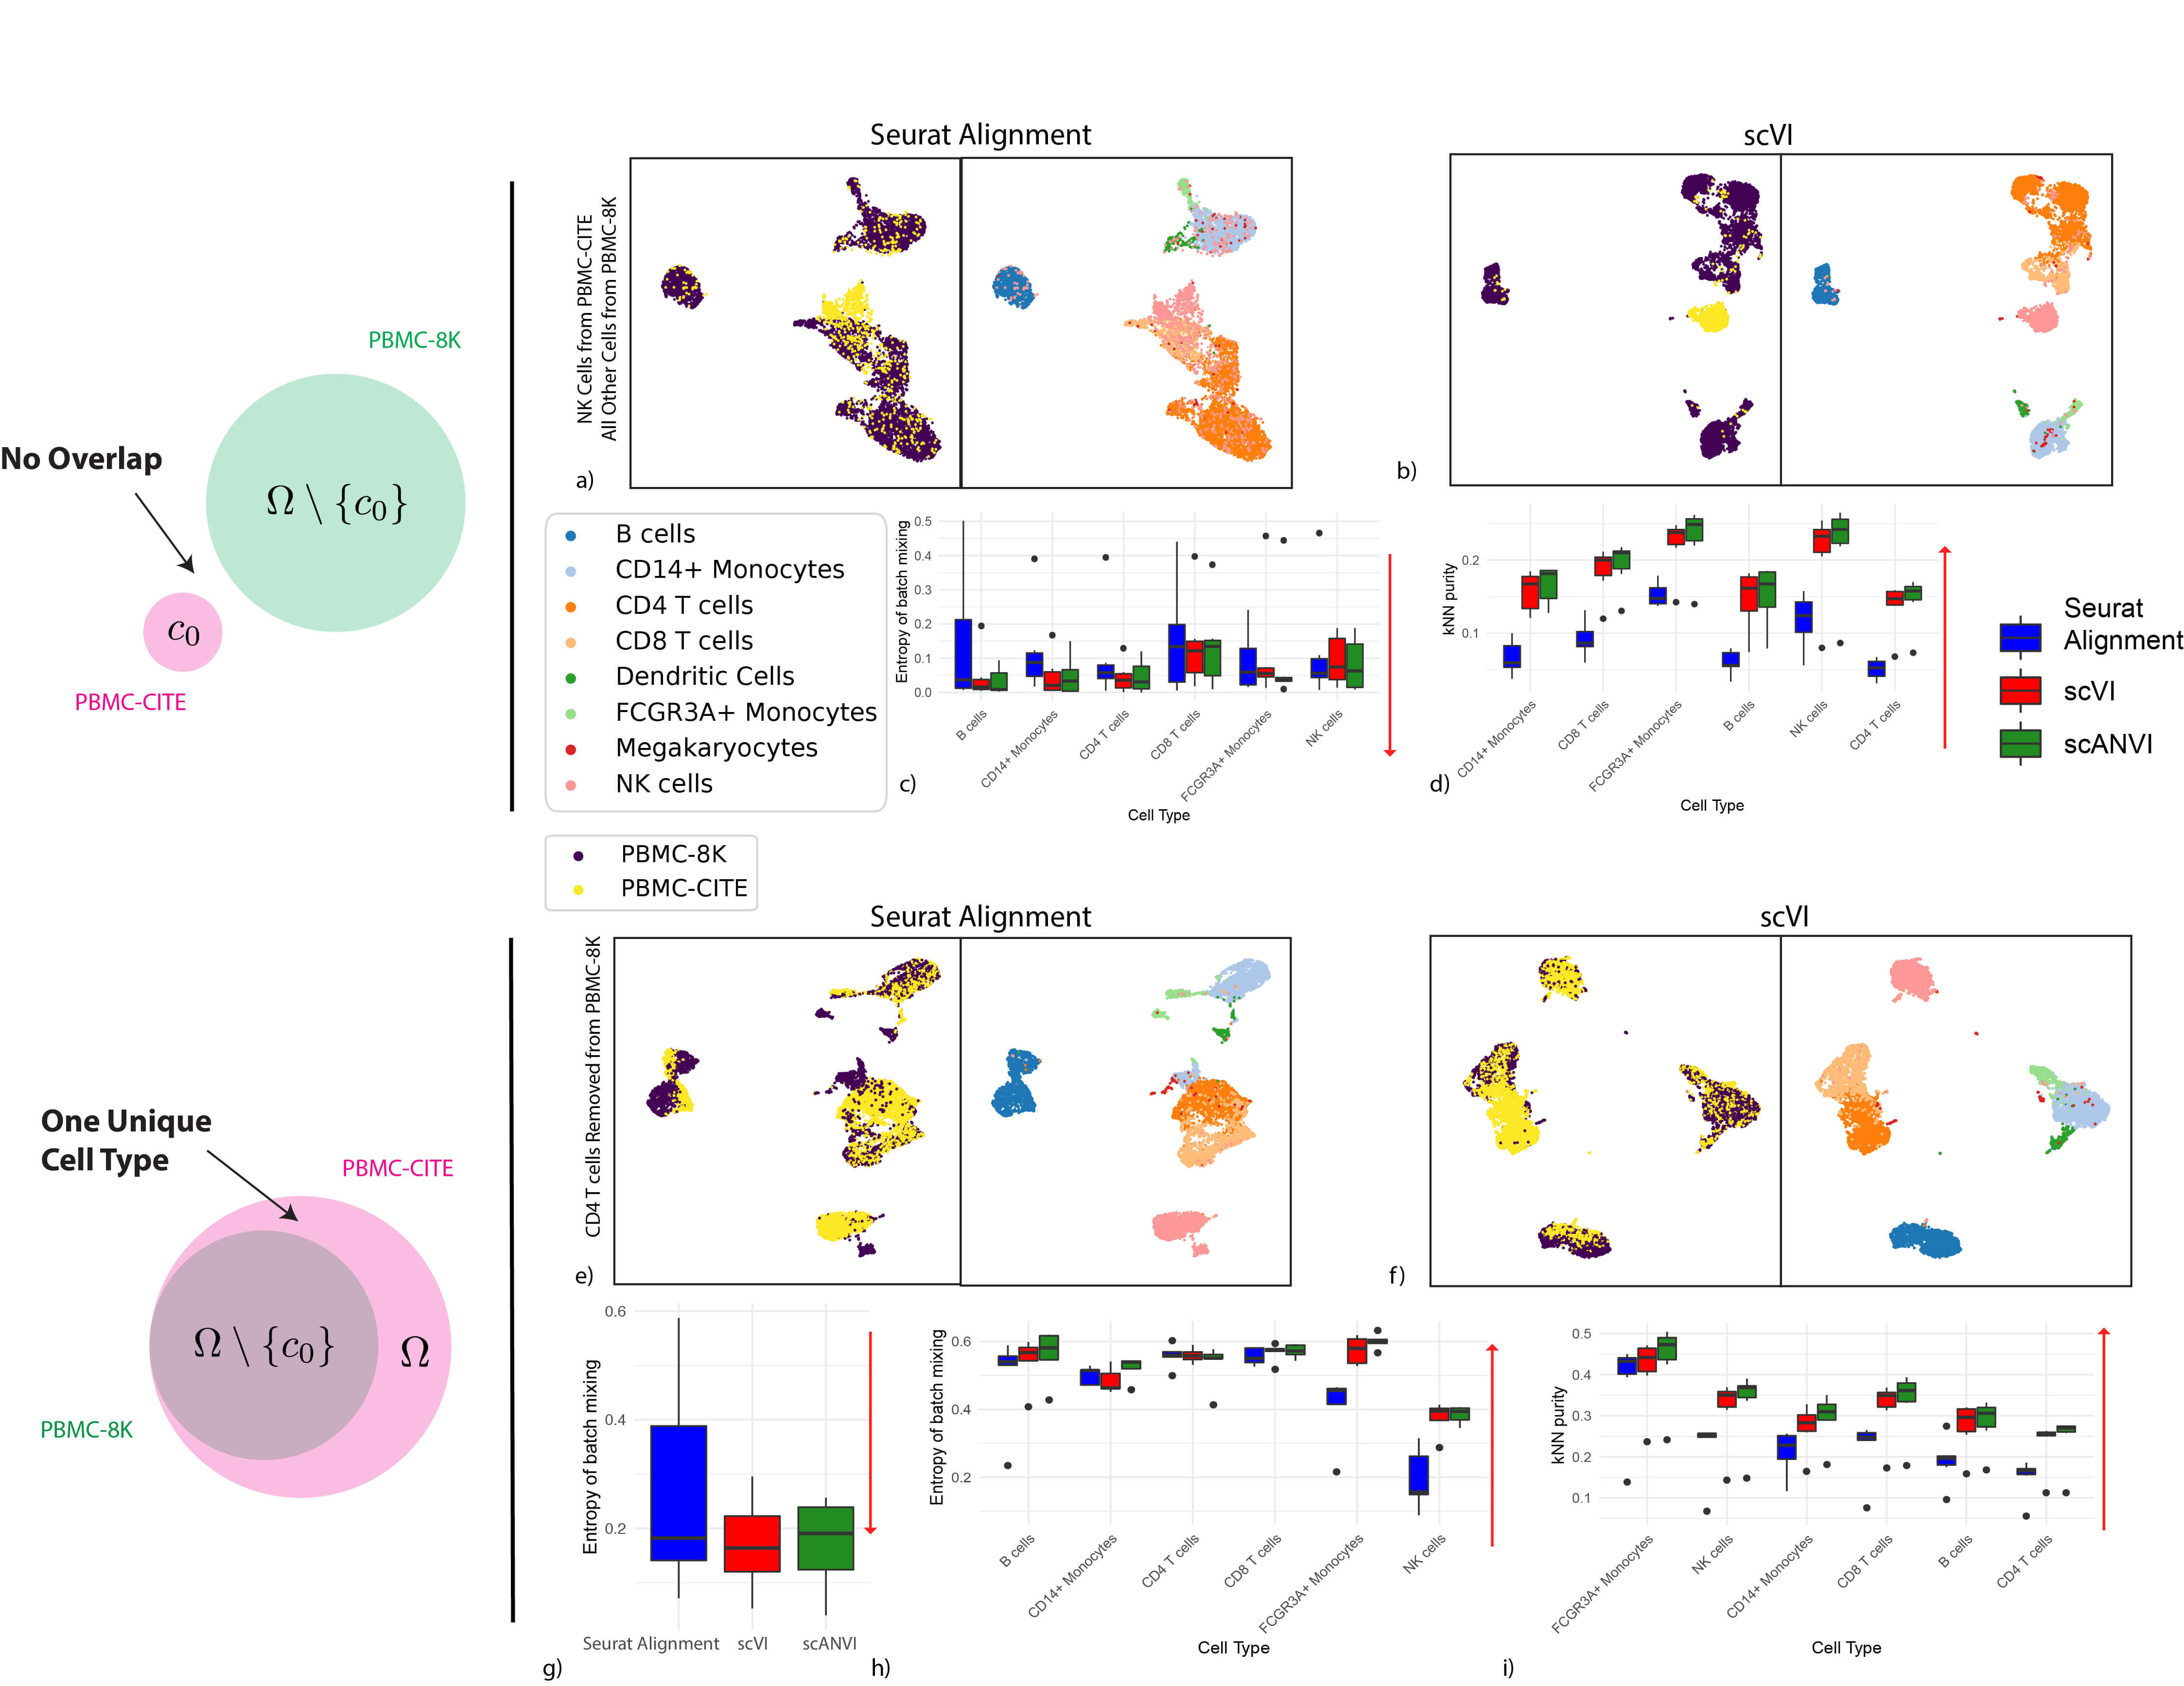
\includegraphics[width=\textwidth]{figures/Fig3.jpg}
\caption[Harmonizing datasets with different cellular composition]{Harmonizing datasets with different cellular composition. $(a-d)$ show the case when no cell type is shared. PBMC-8K contains all cells other than cell type $c_0$ while PBMC-CITE contains only cell type $c_0$. $(a-b)$ UMAP visualization for the case where $c_0$ corresponds to natural killer cells. $(c-d)$ entropy of batch mixing and $k$-nearest neighbors purity, aggregating the six experiments (setting $c_0$ to a different cell type in each experiment). $(e-i)$ show the case when cell type $c_0$ is removed PBMC-8K but not from PBMC-CITE. $(e-f)$ UMAP visualization for the case where $c_0$ corresponds to CD4+ T cells. $(g)$ entropy of batch mixing for the removed cell type. $(h)$ entropy of batch mixing for the remaining cell types. $(i)$ $k$-nearest neighbors purity, aggregating all 6 experiments. Red arrows indicate the desired direction for each performance measure (e.g., low batch entropy is desirable in $(d)$). The boxplots are standard Tukey boxplots where the box is delineated by the first and third quartile and the whisker lines are the first and third quartile plus minus 1.5 times the box height. The dots are outliers that fall above or below the whisker lines.}
\label{scanvirobustness_panel}
\end{figure}


%%%%%%%%%%%%%%%%%%%%%%%%%%%%%%%%%%%%%%%%%%%%%
\subsection{Harmonizing continuous trajectories}
%%%%%%%%%%%%%%%%%%%%%%%%%%%%%%%%%%%%%%%%%%%%%%%%%%%%%%
While so far we considered datasets that have a clear stratification of cells into discrete sub-populations, a conceptually more challenging case is harmonizing datasets in which the major source of variation forms a continuum, which inherently calls for accuracy at a higher level of resolution. 

To explore this, we use a pair of datasets that provides a snapshot of hematopoiesis in mice (HEMATO-Tusi \cite{Tusi2018}, HEMATO-Paul \cite{PAUL2015}; Figure~\ref{scanvicontinuous_panel}). These datasets consist of cells along the transition from common myeloid progenitor cells (Figure~\ref{scanvicontinuous_panel}a-b; middle) through two primary differentiation trajectories myeloblast (top) and erythroblast-megakaryocyte (bottom). Notably, the HEMATO-Tusi dataset contains cells that appear to be more terminally differentiated, which are located at the extremes of the two primary branches. This can be discerned by the expression of marker genes (Figure~\ref{scanvicontinuous_panel}e). For instance the HEMATO-Tusi unique erythroid cell population expresses \textit{Hba-a2} (hemoglobin subunit) and \textit{Alas2} (erythroid-specific mitochondrial 5-aminolevulinate synthase) that are known to be present in reticulocytes \cite{Ery2007,MTAB}. At the other end, the granulocyte subset that is captured only by HEMATO-Tusi expresses \textit{Itgam} and \textit{S100a8}. \textit{S100a8} is a neutrophil specific gene predicted by Nano-dissection \cite{nano2013} and is associated with GO processes such as leukocyte migration associated with inflammation and neutrophil aggregation. \textit{Itgam} is not expressed in granulocyte-monocyte progenitor cells but is highly expressed in mature monocytes, mature eosinophils and macrophages~\cite{papatheodorou2017expression}. We therefore do not expect mixing to take place along the entire trajectory. To account for this, we evaluated the extent of batch entropy mixing at different points along the harmonized developmental trajectory. As expected, we find that in most areas of the trajectory the two datasets are well mixed, while at the extremes, the entropy reduces significantly, using either scVI or Seurat Alignment (Figure~\ref{scanvicontinuous_panel}c). Overall, we observe that scVI compares well in terms of both mixing the differentiation trajectories in each dataset and preserving their original, continuous, structure (Figure~\ref{scanvicontinuous_panel}a-d). 

To validate scANVI in this context as well, we provided it with the categorical labels of cells along the two developmental trajectories, indicating their cell state (Figure~\ref{scanvicontinuous_panel}c-d and Figure~\ref{scanvicontinuousSupp}). Even though this labeling scheme does not explicitly account for the ordering between states, we observe that scANVI is capable of mixing the two datasets, while retaining their original structure, achieving a level of accuracy comparable to that of scVI and better than that of Seurat Alignment. 


\begin{figure}[htp]
\centering
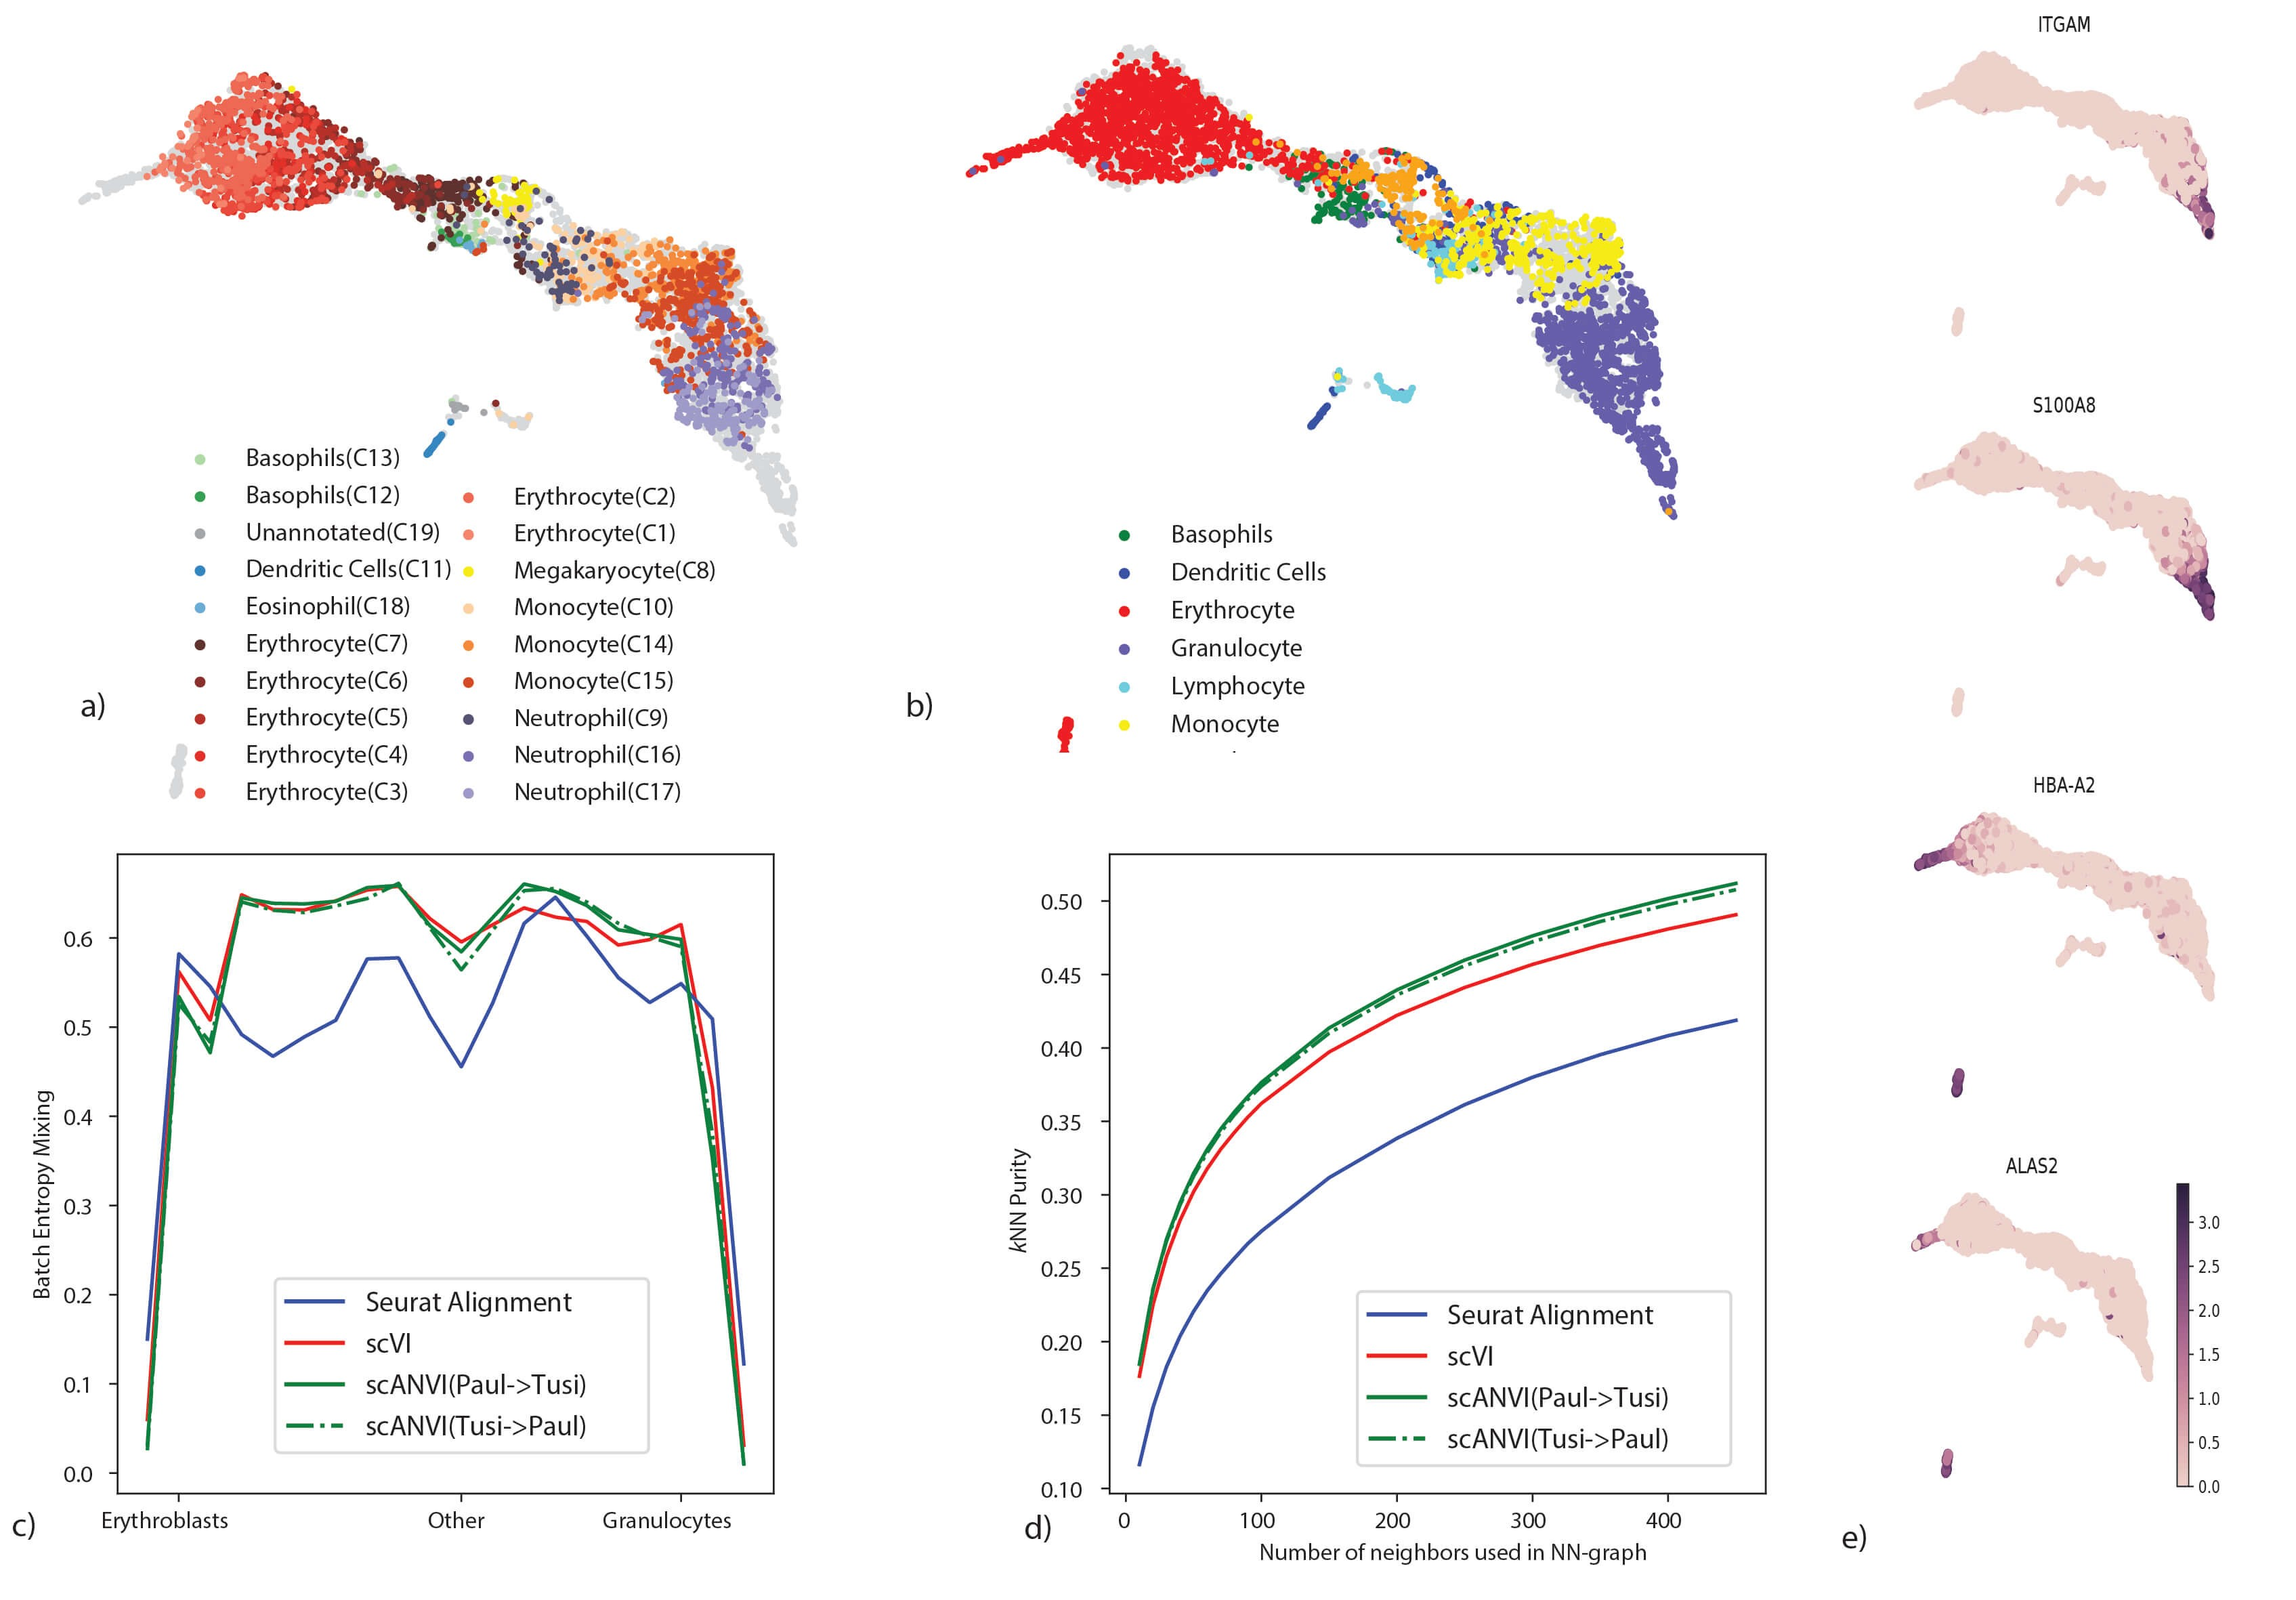
\includegraphics[width=\textwidth]{figures/continuous.jpg}
\caption[Harmonizing developmental trajectories]{Harmonizing developmental trajectories. $(a-b)$ UMAP visualization of the scVI latent space, with cells colored by the original labels from either the HEMATO-Paul $(a)$ or HEMATO-Tusi $(b)$ studies. The cells from the other dataset are colored in gray. $(c)$ Entropy of batch mixing along 20 bins of the HEMATO-Tusi cells, ordered by the potential of each cell. Potential is a pseudotime measure that describes the differentiation state of a cell using the population balance analysis algorithm (center: common myeloid progenitors; moving left: erythrocyte branch; moving right: granulocyte branch). $(d)$ $k$-nearest neighbors purity for scVI, Seurat, and scANVI. $(e)$ Expression of marker genes that help determine the identity of batch-unique cells.} 
\label{scanvicontinuous_panel}
\end{figure}

%%%%%%%%%%%%%%%%%%%%%%%%%%%%%%%%%%%%%%%%%%%%%%%%%%%%%%
\subsection{Rapid integration of multiple datasets}
%%%%%%%%%%%%%%%%%%%%%%%%%%%%%%%%%%%%%%%%%%%%%%%%%%%%%%

To demonstrate the scalability of our framework in the context of harmonizing multiple (and possibly large) dataset, we ran scVI to integrate a cohort of 26 datasets spanning 105,476 cells from multiple tissues and technologies, which was made available by the authors of Scanorama (a method based on truncated singular value decomposition followed by nearest neighbor matching ~\cite{scanorama}). Using the hardware specified in the original paper~\cite{scanorama} (Intel Xeon E5-2650v3 CPU limited to 10 cores with 384 GB of RAM), Seurat Alignment and MNN required over 24 hours, while Scanorama completed its run in 20 minutes. Using a simpler configuration (eight-core Intel i7-6820HQ CPU with 32 GB RAM) along with one NVIDIA Tesla K80 GPU (GK210GL; addressing 24 GB RAM), we found that scVI integrates all datasets and learns a common embedding in less than 50 minutes. This running time is competitive considering the reduced memory availability and the increased complexity of our model, compared to that of Scanorama. Notably, all the downstream analyses, such as annotation, differential expression or visualization can be operated by accessing the latent space or via forward passes through the neural networks. Since these access operations can be conducted very efficiently~\cite{scvi}, the dominant factor, on which we focused our run time analysis, is the time required for model fitting. Considering the results, the latent space of scVI recapitulates well the major tissues and cell types~(Figure~\ref{scanvilarge_scale_panel}), and the position of cells in the latent space provides an effective predictor for the cell type label (Figure~\ref{scanvilarge_scale_panel}).


%%%%%%%%%%%%%%%%%%%%%%%%%%%%%%%%%%%%%%%%%%%%%%%%%%%%%%
\subsection{Transferring cell type annotations between datasets}
%%%%%%%%%%%%%%%%%%%%%%%%%%%%%%%%%%%%%%%%%%%%%%%%%%%%%%

We next turned to evaluate scVI and scANVI in the context of harmonization-based annotation. Here, we test the extent to which annotations from a previously annotated dataset can be used to automatically derive annotations in a new unannotated dataset. For scVI and Seurat Alignment, we derive the annotations by first harmonizing the input datasets and then running a $k$-nearest neighbors classifier (setting $k$ to 10) on the joint latent space, using the annotated cells to assign labels to the unannotated ones. Conversely, scANVI harmonizes the input datasets while using any amount of available labels. The prediction of unobserved labels is then conducted using the approximate posterior assignments $q_\Phi(c \mid x)$ of cell types, directly derived from the model. An alternative approach that we benchmark against was taken by scmap-cluster~\cite{scmap}. scmap directly builds a classifier based on the labeled cells (instead of performing harmonization first) and then applies this classifier to the unlabeled cells. Finally, we also applied the domain adaptation method Correlation Alignment for Unsupervised Domain Adaptation (CORAL,~\cite{sun2016return}). This method was not initially developed for single-cell analysis but is an insightful benchmark from the machine learning literature.

We start by exploring the four dataset pairs in Figure~\ref{benchmarking_panel}, which have been annotated in their respective studies. In each experiment, we ``hide'' the cell type annotations from one dataset and transfer the second dataset labels to the first one. As a measure of performance, we report the weighted accuracy, which is the percent of cells that were correctly assigned to their correct (hidden) label, averaging over all labels. Importantly, the annotations in this first set of case studies were derived computationally. For example, by first clustering the cells, looking for marker genes expressed by each cluster and then assigning labels to the clusters accordingly. This level of annotation therefore makes the prediction problem relatively easy, and indeed, while we find that overall scANVI predicts unobserved labels more accurately, the differences between the methods are mild (Figures~\ref{scanviaccbox} and~\ref{scanvibubble}). Notably, CORAL achieves overall competitive performance except when transferring labels on the MarrowTM pairs, from 10x to Smart-Seq2. In this specific instance, CORAL maps most of the cells to a single label (incidentally, while this label marks cells that are transcriptionally similar, it is defined by the authors as an unknown class ``NA'', corresponding to cells that cannot be confidently assigned or low quality cells according to the authors of \cite{quake2018single}), which might be due to its linear transformation of the feature space. 


To evaluate the accuracy of annotations without the need for computationally-derived labels, we turned to the PBMC-CITE dataset which includes measurements of ten key marker proteins in addition to mRNA~\cite{stoeckius2017simultaneous}, and the PBMC-sorted dataset~\cite{zheng2017massively}, where cells were collected from bead purifications for eleven cell types (Table~\ref{scanvipbmc-pure-celltypes}). We applied scVI and scANVI to harmonize and annotate these two datasets along with a third dataset of PBMC (PBMC-68K~\cite{zheng2017massively}). Our analysis contains a combined set of $n=169,850$ cells from the three datasets altogether. To generate a realistic scenario of cell type annotation, we only provide access to the experimentally-based labels from the PBMC-sorted dataset (Figure~\ref{scanviconcordance_panel}a-c). As an additional benchmark, we also evaluate Seurat Alignment, which was tested after removal of a randomly selected subset ($40 \%$) of the two large datasets (PBMC-68K and PBMC-sorted) due to scalability issues. Considering our harmonization performance measures (i.e., retainment of the original structure and batch mixing), we observe as before that scVI and scANVI perform similarly and compare favorably to Seurat Alignment. We then evaluated the accuracy of assigning unobserved labels, focusing on the PBMC-CITE dataset. Instead of using the labels from the original PBMC-CITE study as ground truth (which were computationally derived), we used the protein data, which provides an experimentally-derived proxy for cell state. To this end, we quantified the extent to which the similarity between cells in the harmonized mRNA-based latent space is consistent with their similarity at the protein level. We first computed the average discrepancy (sum of squared differences) between the protein measurements in each cell and the average over its $k$-nearest neighbors. As a second measure we computed for each PBMC-CITE cell the overlap between its $k$-nearest PBMC-CITE neighbors in the harmonized mRNA-based space and in the protein space. We then report the average across all cells in Figure~\ref{scanviconcord_supplement}. Evidently, scANVI outperformed both scVI and Seurat Alignment for a wide range of neighborhood sizes, providing a representation for the mRNA data that is more consistent with the protein data (Figure~\ref{scanviconcordance_panel}c).


\begin{table}
\centering
\begin{small}
\begin{tabular}{lc}
    \toprule
\textbf{Cell Types}        & \textbf{\# cells} \\
\midrule
\textbf{B cells}           & 10,085   \\
\textbf{CD14+ Monocytes}   & 2,612    \\
\textbf{CD34+ cells}       & 9,232    \\
\textbf{CD4 T cells}       & 11,213   \\
\textbf{CD56 NK cells}     & 8,385    \\
\textbf{CD8 T cells}       & 10,209   \\
\textbf{Memory T cells}   & 10,224   \\
\textbf{Naive CD8 T cells} & 11,953   \\
\textbf{Naive T cells}     & 10,479   \\
\textbf{Regulatory T cells}     & 10,263   \\
\bottomrule
\end{tabular}
\end{small}
\caption{Cell types present in the PBMC-sorted dataset.}
\label{scanvipbmc-pure-celltypes}
\end{table}
 

\begin{figure}
\centering
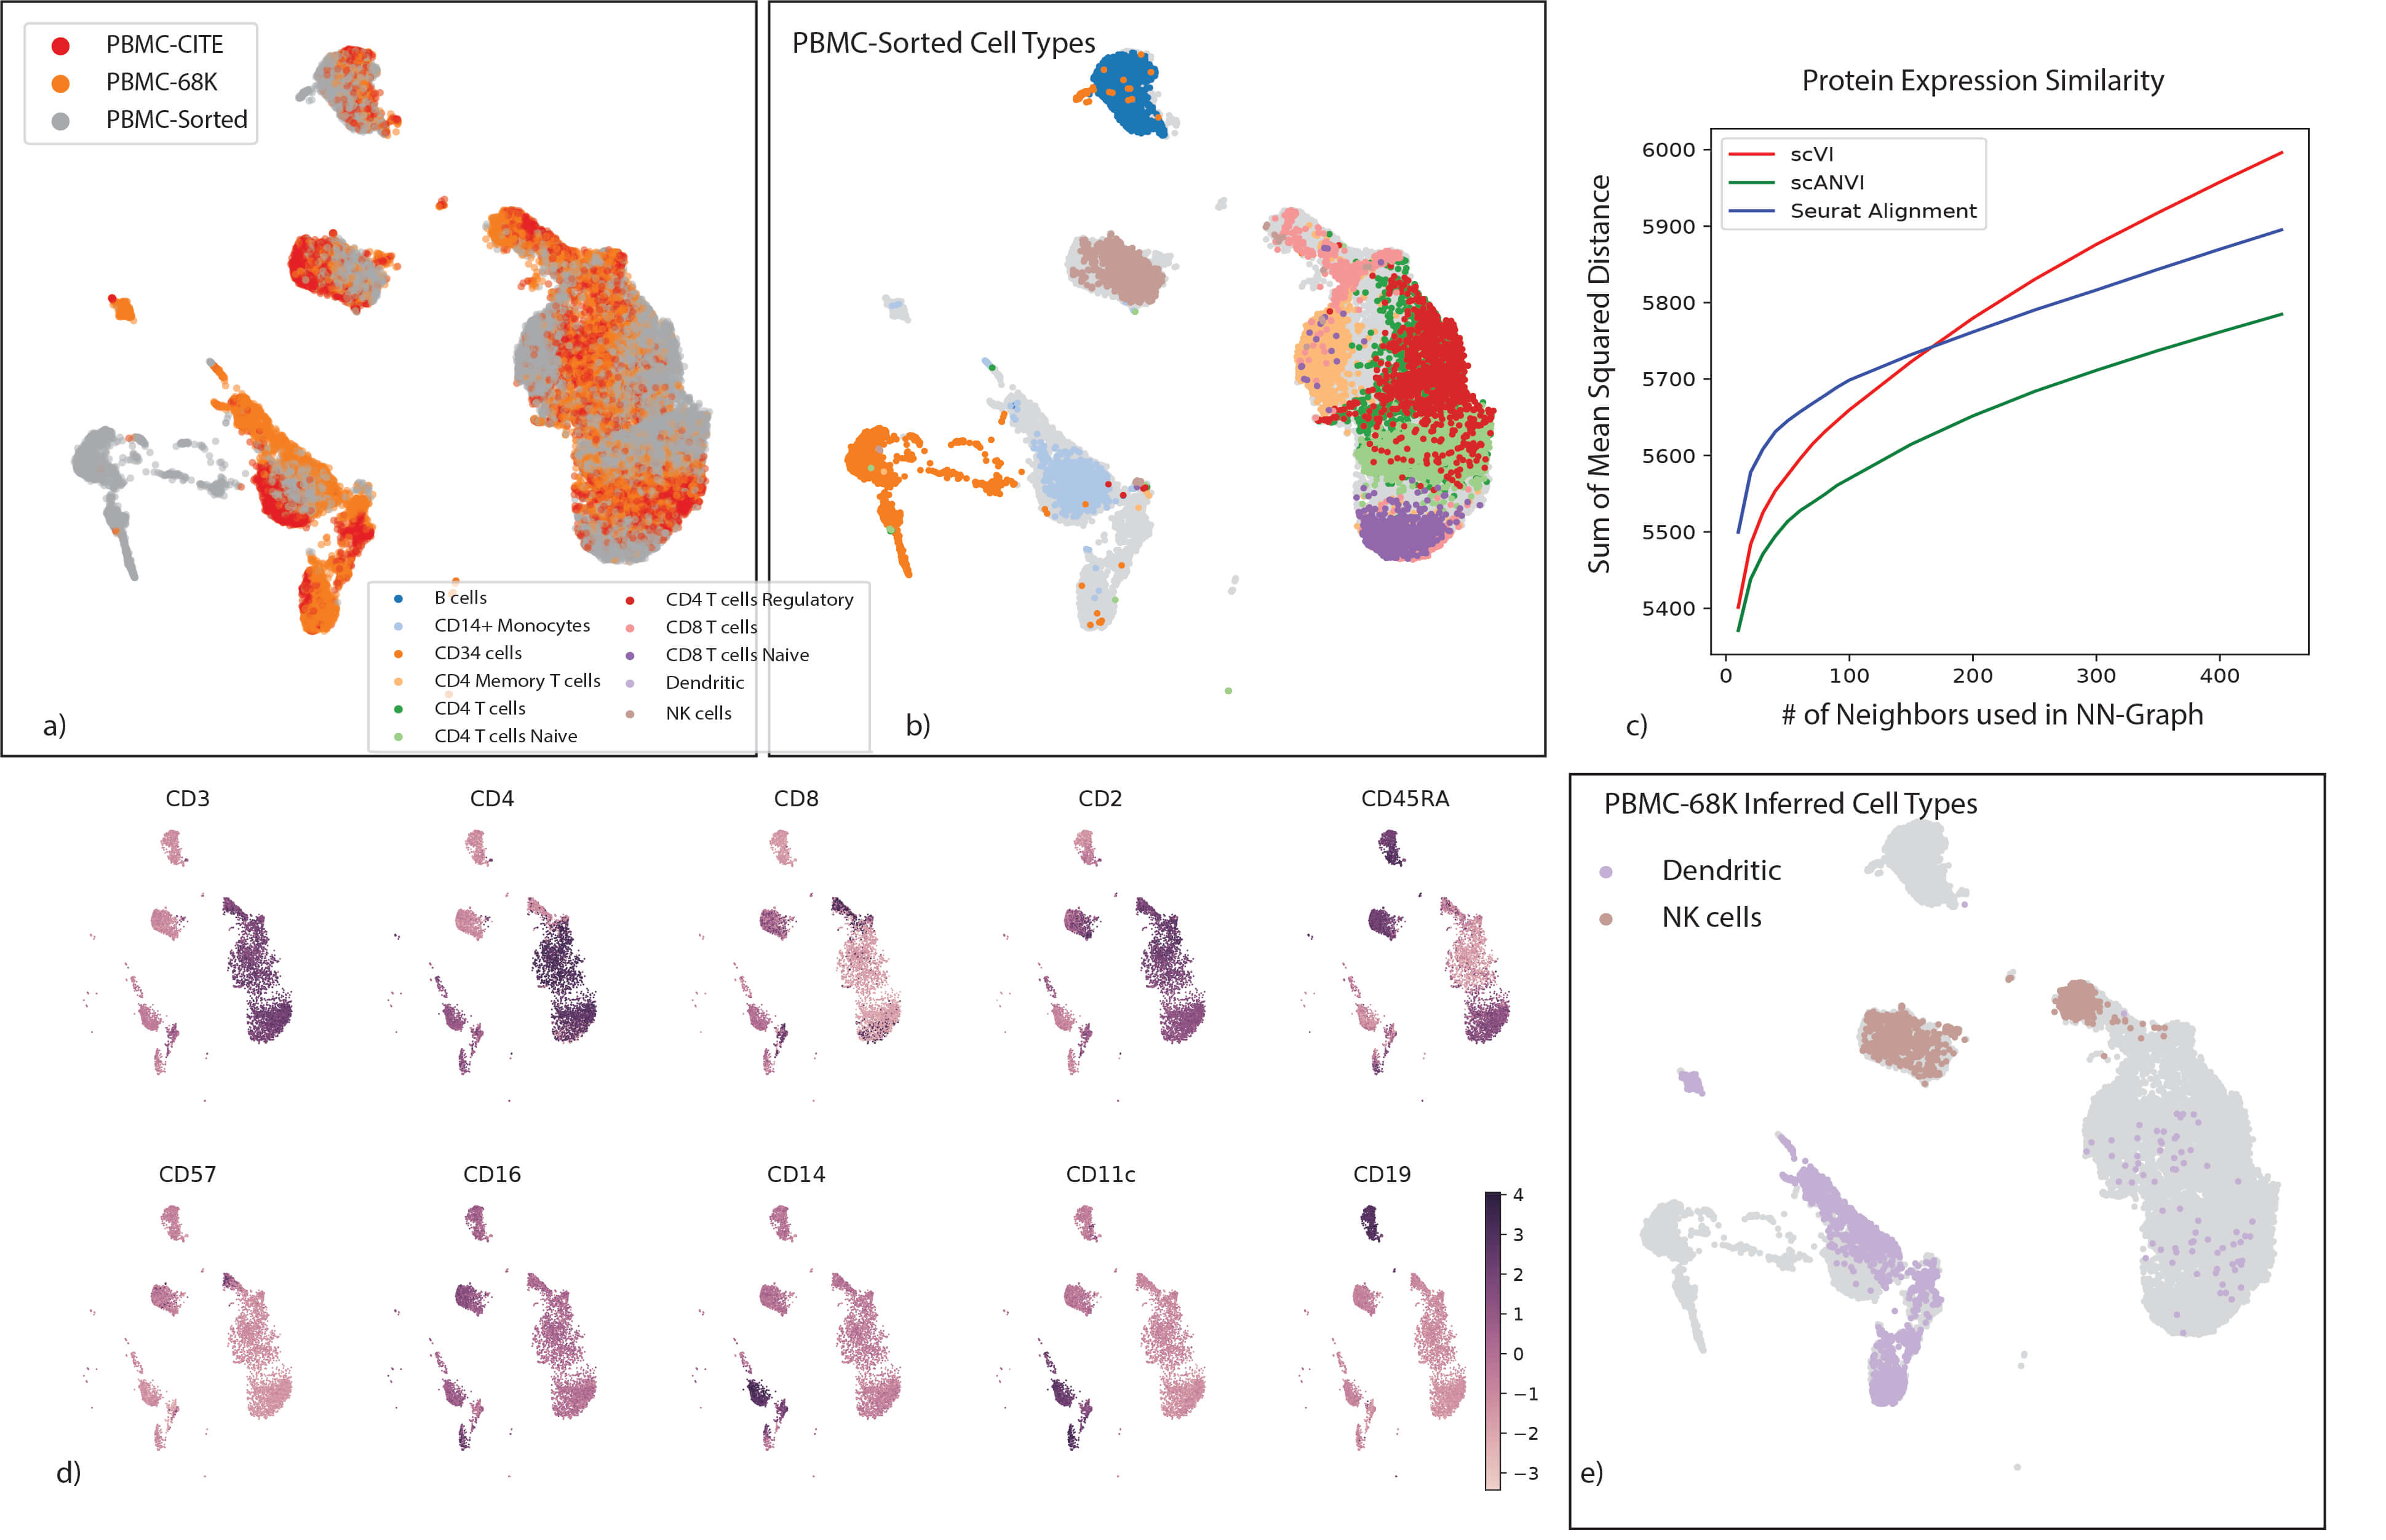
\includegraphics[width=\textwidth]{figures/labels_concored.jpg}
\caption[Validation of cell type annotations using additional metadata]{Validation of cell type annotations using additional metadata. (a-b) UMAP plot of the scANVI latent space inferred for three harmonized datasets: PBMC-CITE, PBMC-sorted, and PBMC-68K. Cells are colored by the dataset of origin $(a)$ and the PBMC-sorted labels $(b)$. Cells from the PBMC-CITE and PBMC-68K are colored in gray in $(b)$. (c) The consistency of the harmonized PBMC-CITE mRNA data with the respective protein measurements, evaluated by mean squared error and for different neighborhood size. Lower values indicate higher consistency. $(d)$ UMAP plot of the scANVI latent space, where cells are colored by normalized protein measurement. Only PBMC-CITE cells are displayed. $(e)$ UMAP plot of the scANVI latent space, with cells from the PBMC-68k dataset colored according to their original label. For clarity of presentation, only cells originally labeled as dendritic cells or natural killer cells are colored. Evidently, a large number of these cells are mapped to a cluster of T-cells (right side of the plot).}
\label{scanviconcordance_panel}
\end{figure}


%%%%%%%%%%%%%%%%%%%%%%%%%%%%%%%%%%%%%%%%%%%%%%%%%%%%%%
\subsection{Cell type annotation in a single dataset based on ``seed'' labels}
%%%%%%%%%%%%%%%%%%%%%%%%%%%%%%%%%%%%%%%%%%%%%%%%%%%%%%
An important variant of the annotation problem lies within the context of an \textit{ab initio} labeling of a single dataset where only a subset of the cells can be confidently annotated based on the raw data. This increasingly prevalent scenario may result from limited sensitivity of the scRNA-seq assay, where marker genes may only be confidently observed in a small subset of cells. One common way to address this problem is to compute some form of a distance metric between cells (e.g., after embedding with scVI or using Seurat PCA) and then assign labels based on proximity to annotated cells \cite{zheng2017massively}. To benchmark our methods, we consider two such predictors: the first is clustering the cells and taking a majority vote inside each cluster, and the second is taking the majority vote of the $k$-nearest neighbors around each unannotated cell ($k=10$). While these approaches are quite straightforward, their accuracy might suffer when the data do not form clear clusters~\cite{Tusi2018}, or when differences between labels are too subtle to be captured clearly by a transcriptome-wide similarity measure. To address these issues, scANVI takes an alternative approach, namely learning a latent embedding that is guided by the available labels, and then producing posterior probabilities for assigning labels to each cell. 

As a case study, we compiled a dataset consisting of several experimentally sorted and labeled subsets of T cells from the PBMC-sorted dataset, including CD4 memory, CD4 naive, CD4 regulatory and CD8 naive. To make our analysis more realistic, we assume that the labels are completely unknown to us and therefore assign each T cell to its respective subset using marker genes (12 altogether):
\begin{itemize}
    \item \textbf{CD4 regulatory}: \textit{GITR}$^+$ \textit{CTLA4}$^+$ \textit{FOXP3}$^+$ \textit{CD25}$^+$ \textit{S100A4}$^-$\textit{CD45}$^-$\textit{CD8B}$^-$
    \item \textbf{CD4 naive}: \textit{CCR7}$^+$ \textit{CD4}$^+$ \textit{S100A4}$^-$\textit{CD45}$^-$\textit{FOXP3}$^-$\textit{IL2RA}$^-$\textit{CD69}$^-$
    \item \textbf{CD4 memory}: \textit{S100A4}$^+$ \textit{CD25}$^-$\textit{FOXP3}$^-$\textit{GITR}$^-$\textit{CCR7}$^-$
    \item \textbf{CD8 naive}: \textit{CD8B}$^+$ \textit{CCR7}$^+$ \textit{CD4}$^-$
    \end{itemize}
Notably, several important biomarkers (\textit{CD4}, \textit{CTLA4}, and \textit{GITR}) are detected in less than $5 \%$ of the cells. This renders their use for annotation not straightforward. Furthermore, many of these biomarkers are sparsely expressed to the extent that they are likely to be filtered out in the gene selection step of most harmonization procedures (Figure~\ref{scanviscanvi_panel}a). 


To analyze this dataset, we first computed a signature score for each cell and for each label (i.e., T cell subset) using the scaled raw expression values of the respective marker genes. We then designated the top $50$ scoring cells in each subset as the seed set of cells that are confidently annotated for that subset (Figure~\ref{scanviscanvi_panel}b). Reassuringly, this partial annotation is in agreement with the experimentally-derived cell type labels available for this dataset (Figure~\ref{scanviscanvi_panel}c). However, this dataset does not form clear clusters, and in particular the seed sets of cells are not well separated. Such an observation makes clustering-based approaches potentially less precise. Indeed, using $k$-means clustering on the scVI and Seurat PCA latent space, we find that $74 \%$ and $72\%$ of the cells were assigned with their correct label. Similar analysis with two additional popular clustering algorithms (DBSCAN~\cite{dbscan} and PhenoGraph~\cite{Levine_PhenoGraph_2015}) further emphasizes the challenge of a cluster-based approach on this data. Specifically, DBSCAN does not partition the data into more than one cluster (scanning through a large number of parameter values), and PhenoGraph predicts 9 clusters and achieves an accuracy of $41 \%$ (Figure~\ref{scanviscanviClustering}). 

%Chenling: Fig 6: panel B needs to scVI

Consistent with these results, the application of a $k$-nearest neighbors classifier resulted in a similar level of accuracy in the Seurat PCA latent space ($71 \%$), which is slightly improved when replacing it with the scVI latent space ($73 \%$; Figure~\ref{scanviscanviClustering}). Conversely, after fitting the scANVI model based on this partial labeling, the annotation posterior $q_\Phi(c \mid z)$ (Figure~\ref{scanviscanvi_panel}d) provides a substantially more accurate cell type assignment, with $84 \%$ of cells annotated correctly. 

While scANVI has been designed to handle discrete (but not continuous) labels, we hypothesized that gradual transition between cell states may still be captured by the uncertainty of label assignment. We tested it using simulated data~\cite{symsim} that consists of a set of ``end-point'' states along with intermediary states that connect them (Figure~\ref{scanvisymsim_cont}a). We provided labels only to end-point cells, and investigated the label assignment scores calculated for the intermediary cells. We find that scANVI provides a range of assignment probability values and that these values are proportional to the distance from the respective end points (Figure~\ref{scanvisymsim_cont}b-g). Conversely, the scores provided by scmap tend to be more extreme (Figure~\ref{scanvisymsim_cont}h-i), thus less reflecting the continuous nature of the data.



\begin{figure}[ht]
\centering
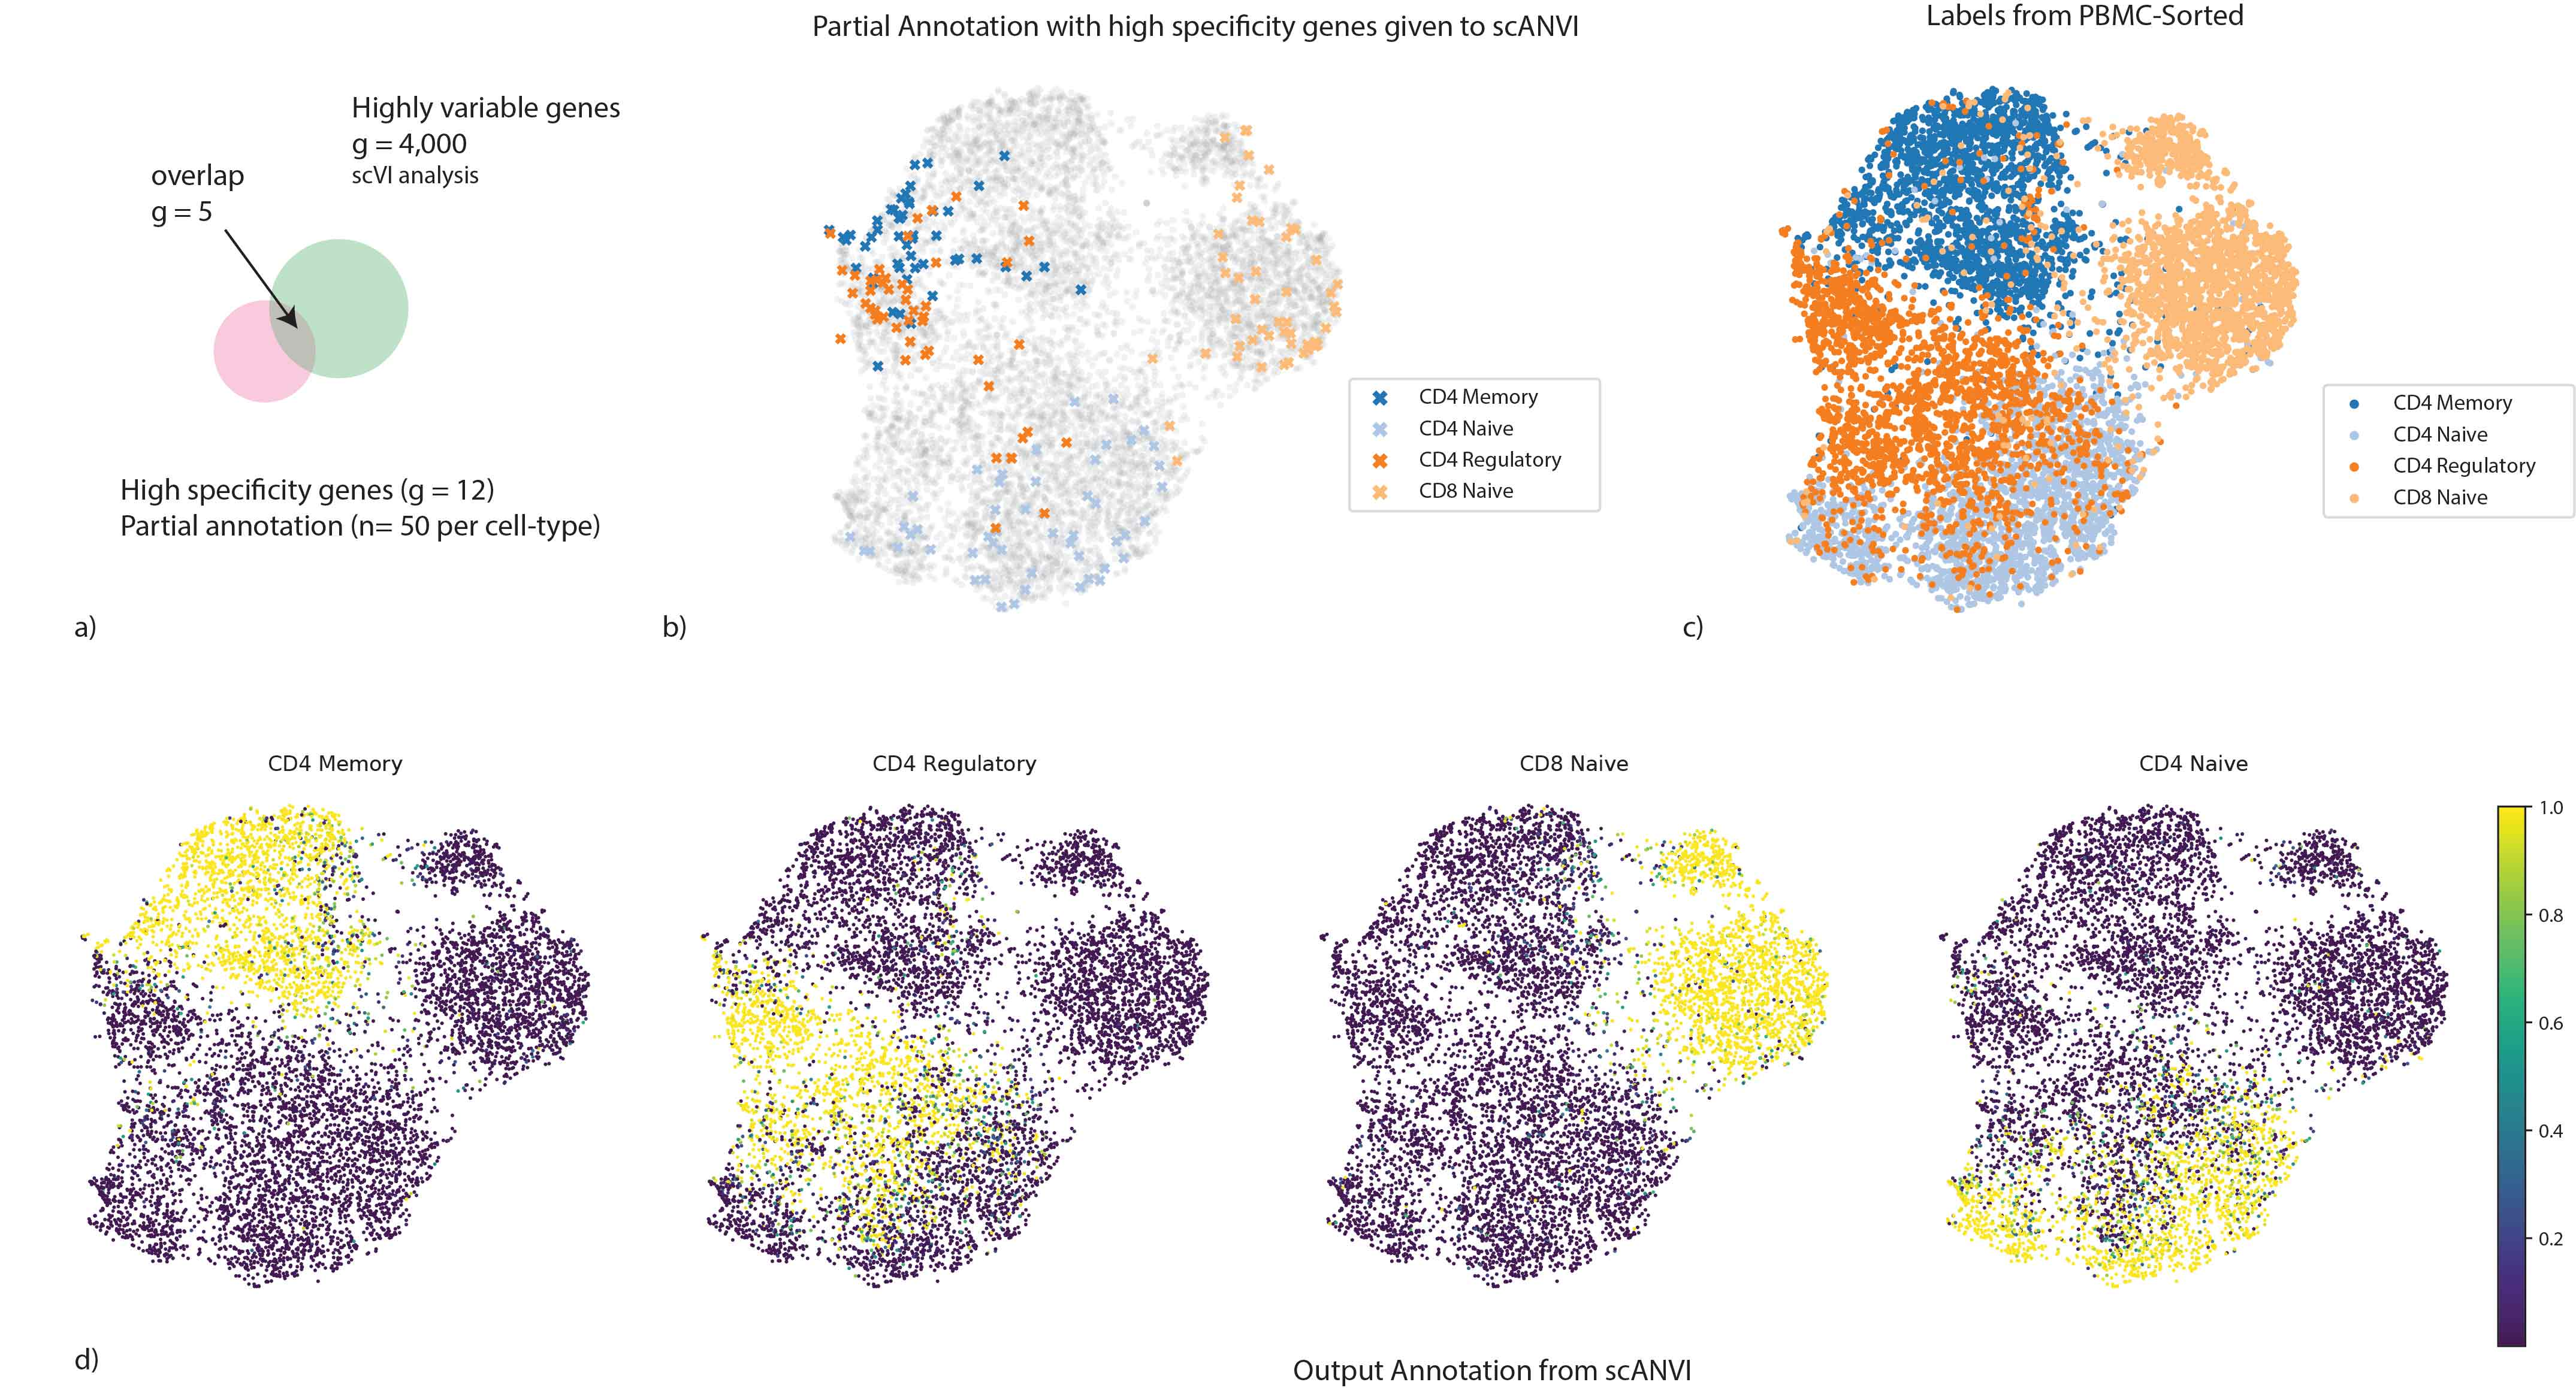
\includegraphics[width=\textwidth]{figures/scanvi.jpg}
\caption[Cell type annotation in a single dataset using ``seed'' labeling]{Cell type annotation in a single dataset using ``seed'' labeling. $(a)$ discrepancies between marker genes that can be used to confidently label cells and highly variable genes in scRNA-seq analysis. $(b-d)$ UMAP plot of the scVI latent space. $(b)$ Seed cells are colored by their annotation (using known marker genes). $(c)$ PBMC-sorted cell type labels from the original study based on marker-based sorting $(d)$ The posterior probability of each cell being one of the four T cell subtypes obtained with scANVI.}
\label{scanviscanvi_panel}
\end{figure}


%%%%%%%%%%%%%%%%%%%%%%%%%%%%%%%%%%%%%%%%%%%%%%%%%%%%%%
\subsection{Cell type taxonomy and hierarchical classification with scANVI}
%%%%%%%%%%%%%%%%%%%%%%%%%%%%%%%%%%%%%%%%%%%%%%%%%%%%%%
Another subtle yet important variation of the annotation problem is when the labels are not mutually exclusive but rather form a taxonomy of cell types or states. To effectively annotate cells in this setting, we extended scANVI to perform hierarchical classification, which as before we carry out from first principles, relying on probabilistic graphical models. 

\subsubsection{Hierarchical classification of cells onto a cell type taxonomy}
For hierarchical label propagation in scANVI, we propose a extension of the formerly presented model by modifying the variable $c_n$ to be a tuple where each entry denotes the label at a given level of the hierarchy. Our approach is similar to previous work in robustness to noisy labels~\cite{goldberger2016training} and hierarchical multi-labels flavors of classification problems~\cite{pmlr-v80-wehrmann18a}. We now detail the case for a depth of level two in though our approach can in principle be adapted to arbitrary depths. In our setting, the taxonomy needs to be hard-coded and known \textit{a priori}.

We do not modify the generative model but only the structure of the variable~$c_n$ in the variational distribution. Notably, we formally pose: 
\begin{align}
    c_n = (y_n, y^g_n) \in \{0, \ldots, C\} \times \{0, \ldots, C^g\},
\end{align} 
where $C$ denotes the number of cell types and $C^g$ the number of cell type groups. The parametrization of the full variational distribution $q(c \mid z) = q(y, y^g \mid z)$ must be further defined. For this, we notice that the prior taxonomy knowledge encapsulates whether the assignment $(y^g, y) = (i, j)$ is biologically possible (i.e cell type $i$ is a sub-population of group cell type $j$). We encode this biological compatibility into a parent function $\pi: \{0, \ldots, K\} \rightarrow \{0, \ldots, K^g\}$ that maps a cell type to its parent in the hierarchy. We note for simplicity:
\begin{align}
    q(y_i, y^g_j \mid z) = q(y = i, y^g = j \mid z).
\end{align}
We then use two neural networks $f$ and $f_g$ (with softmax non-linearities) to map the latent space to the joint approximate posterior $ q(y, y^g \mid z)$ with the following rules:
\begin{align}
\begin{split}
q(y_i, y^g_j \mid z) &=
\begin{cases}
f_i(z) & \text{ if } \pi(i) = j,\\
0 & \text{ otherwise}.\\
\end{cases} \\
q(y^g_j \mid z) &= f^g_j(z).
\end{split}
\end{align}
Then, we can derive the marginal probability over finer cell types classes using the chain rule and Bayes rule: 
\begin{align} 
    q(y_i \given z) &=  q(y_i \given y_{\pi_i} , z) q(y_{\pi_i} \given z)\\
     &= \frac{q(y_i, y_{\pi_i} \given  x)}{q(y_{\pi_j} \given  x)} q(y_{\pi_i} \given z)\\
    & = \frac{q(y_i, y_{\pi_i} \given  x)}{\sum\limits_{j \in c(\pi_i)} q(y_j, y_{\pi_j} \given  x)}q(y_{\pi_i} \given z)\\
    & = \frac{f_i(z)}{\sum\limits_{j \in c(\pi_i)} f_j(z)}f^g_{\pi_i}(z),
\end{align}
where $c(\pi_i)$ denotes the set of children of node $i$ children.


\subsubsection{Dataset}
To demonstrate this extended version, we use a dataset of the mouse nervous system~\cite{zeisel2018} that was annotated using a cell type taxonomy with several levels of granularity. At the lowest (most granular) level, the cells are stratified into 265 cell sub-types. At the second lowest level of granularity these 265 subtypes are grouped into 39 subsets, each corresponding to a more coarse definition of a cell type. The multi-level labels are generated through an iterative process that is described in detail in the original publication~\cite{zeisel2018}. The clustering was performed with strict quality filters, takes into account anatomical information and were validated at different levels using existing scRNAseq dataset, osmFISH, RNAscope and others. The cell types taxonomy is derived differently for each level and the details can be found in the original publication. Cell type clusters were obtained by Louvain clustering on a multiscale $k$-nearest neighbors graph and DBSCAN. The first level separates neurons and non-neuronal cells. The second level separates peripheral neuronal system from central neuronal system. The third layer separates anterior posterior domain, and the fourth layer is split by excitatory versus inhibitory neurotransmitter. At this level, all cells are divided into 39 subsets, each corresponding to a coarse cell type definition. Then, within each subset the authors defined ($N$=28) enriched genes and used linkage (correlation distance and Ward method) to construct the dendrogram.

\subsubsection{Results}
We evaluate the ability of scANVI as well as the competing methods at inferring the most granular level of labels when provided with partial ``seed'' annotation --- namely label information for 5 randomly selected cells per label (which accounts for an overall of $0.8 \%$ of the cells). We first observe that Seurat PCA followed by a $k$-nearest neighbors classifier provides a weighted accuracy of $23 \%$ (averaging over all cell types). While this might seem like a low accuracy, it is in fact far from trivial since the expected weighted accuracy of a random classifier or a constant predictor is of around $\nicefrac{1}{265} \approx 0.3 \%$. Such low numbers are due to the high number of labels at this highly granular scale. scVI provides a substantially better, yet still low level of accuracy at $32 \%$. Interestingly, when scANVI is used without accounting for hierarchy, its performance is similar to the unsupervised scVI (at $32 \%$), which might result from very large number of labels that may require hyperparameter tuning (e.g., increasing the number of classifier training epochs). However, when we take the hierarchy of the labels into account, the performance of scANVI increases to $37 \%$, thus outperforming the other methods by a significant margin. Notably, while we tested the extrapolation of seed labeling and the hierarchical mode only in the context of a single dataset, this variation of the scANVI model can also be directly applied in the context of multiple datasets (i.e., transferring hierarchical annotations between datasets).


%%%%%%%%%%%%%%%%%%%%%%%%%%%%%%%%%%%%%%%%%%%%%%%%%%%%%%
\subsection[Differential expression in harmonized datasets]{Hypothesis testing in harmonized datasets: the case of differential expression}
%%%%%%%%%%%%%%%%%%%%%%%%%%%%%%%%%%%%%%%%%%%%%%%%%%%%%%


\begin{figure}[htp]
\centering
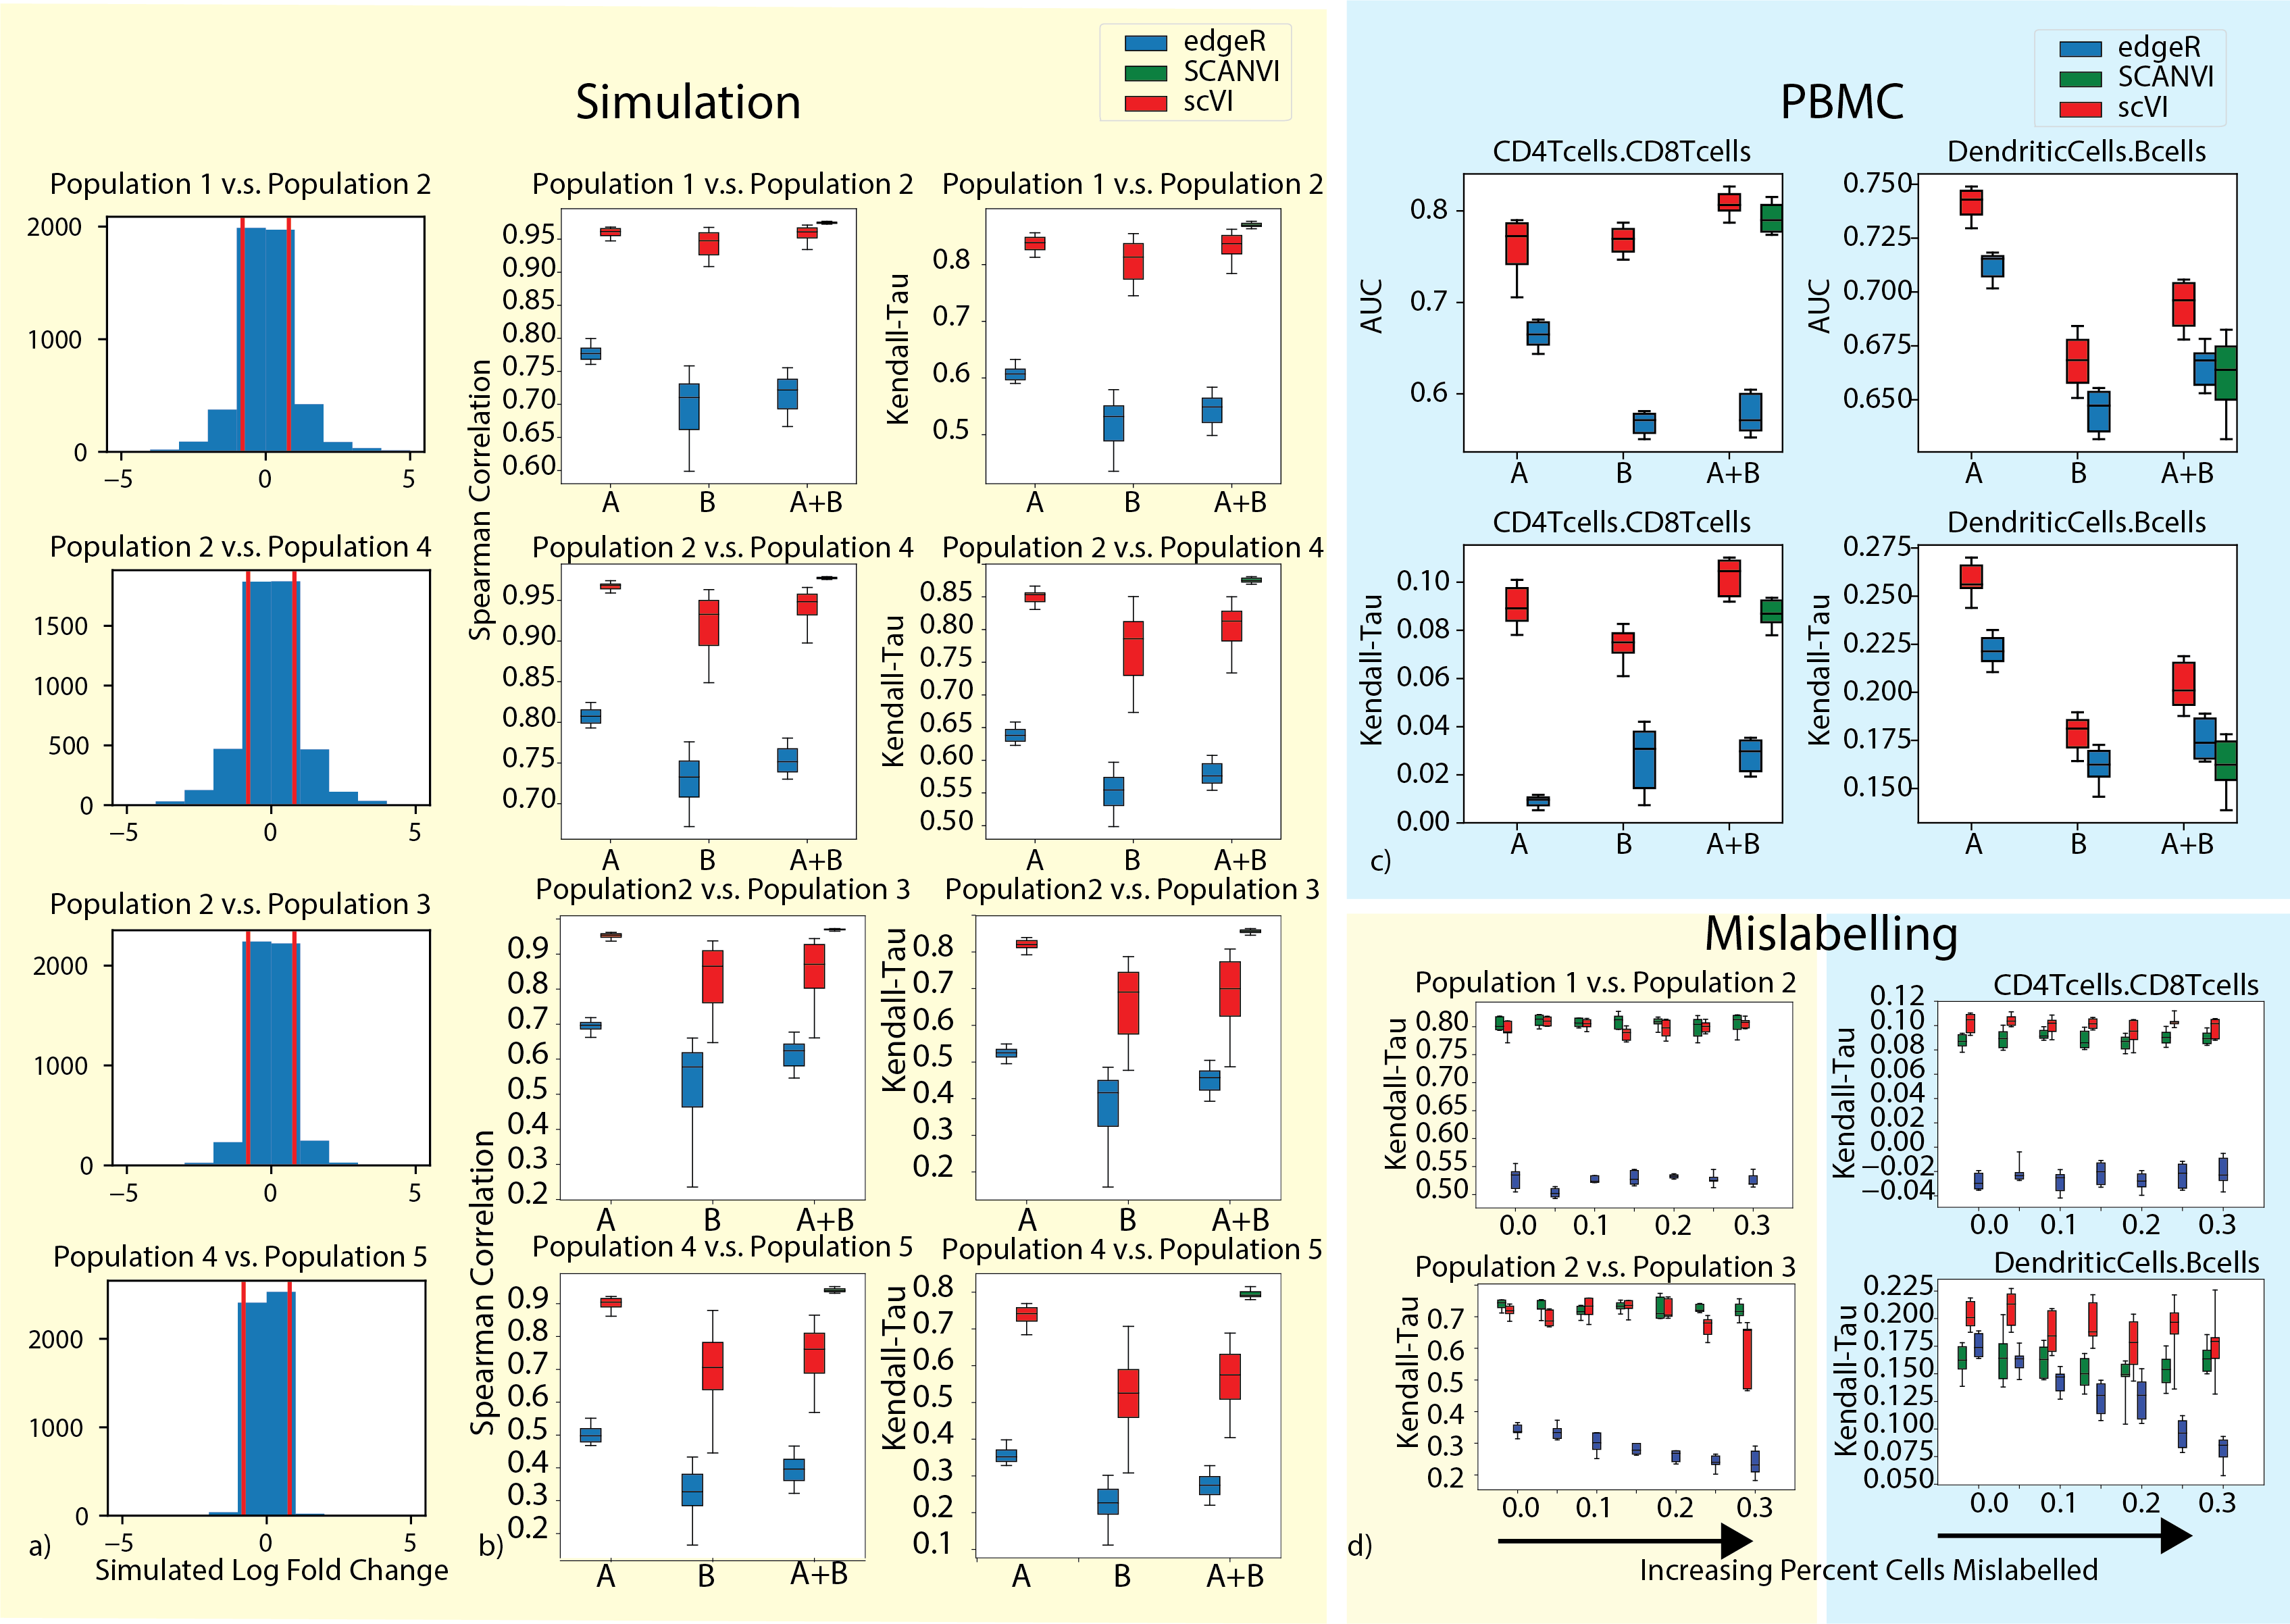
\includegraphics[width=0.8\textwidth]{figures/DE_maintext.png}
\caption[Differential Expression on multiple datasets with scVI]{Differential Expression on multiple datasets with scVI. $(a)$ distribution of true log fold change between all pairs of cell types for the simulated data. The pairs of cells are chosen to represent different levels of distance on the tree as in Figure~\ref{scanvisimulations_panel}a. The pairs of population from most distant to least distant are `12', `24', `23', `45'. 
$(b)$ Evaluation of consistency with rank correlation and Kendall-Tau is shown for comparisons of multiple pairs of cell types in the simulated data. 
$(c)$ Evaluation of consistency with the AUROC and Kendal Tau metric is shown for comparisons of CD4 vs CD8 T cells and B cells vs Dendritic cells on the PBMC-8K only (A), the PBMC-68k only (B) and the merged PBMC-8K / PBMC-68K (A+B) for scVI and edgeR. Error bars are obtained by multiple subsampling of the data to show robustness.  boxplots are standard Tukey boxplots where the box is delineated by the first and third quartile and the whisker lines are the first and third quartile plus minus 1.5 times the box height. The dots are outliers that fall above or below the whisker lines.
$(d)$ Mislabeling experiment in differential expression in both the SymSim simulated datasets and in the PBMC8K and PBMC68K dataset. The top row shows differential expression results for the correctly labeled population pair (Population 1 v.s. Population 2 in simulated dataset and CD4 T cells v.s. CD8 T cells in PBMC dataset. The bottom row shows differential expression results for the mislabelled population pair ( Population 2 v.s. Population 3 in simulated dataset and Dendritic Cells v.s. B cells in PBMC dataset). For all, x-axis represents the proportion of flipped labels. }
\label{scanvide_panel}
\end{figure}

With their probabilistic representation of the data, scVI and scANVI each provide a natural way of performing various types of hypotheses testing. This is different from other approaches~\cite{MNN,seurat,LIGER,scanorama,SEURAT3} where the dataset alignment procedures do not carry direct probabilistic interpretation, and the resulting harmonized data can thus not be directly used for these purposes.

\subsubsection{Bayesian differential expression with scANVI}
Contrary to scVI, scANVI doesn't need to rely on specific cells for differential expression since labels are given during the training. We still use the generative model but with the following probability for $p(\mathcal{H}_1^g \mid c_a, c_b)$ where $c_a$ (resp. $c_b$) is the first (resp. second) cell type of interest:
\begin{align}
p(\mathcal{H}_1^g \mid c_a, c_b) = \sum_s\int \mathds{1}_{f_w^g(z_a, s) \leq f_w^g(z_b, s) }p(s)dp(z_a \mid u_a, c_a)dp(z_b \mid u_b, c_b)dp(u_a)dp(u_b).
\end{align}
Notably, we draw here data from the prior distribution and not the posterior for given cells. As a consequence, these Bayes factors can be approximated in a unbiased fashion using a naive Monte Carlo estimator. We noticed in the case of the real dataset that the aggregate posterior on $u$ might not perfectly match the prior for rare cell types. Consequently, we replaced the prior by the aggregate posterior for all the analyses in this chapter. 

\subsubsection{Dataset}


To demonstrate this, we focus on the problem of differential expression. As a first case study, we use two of the PBMC datasets (PBMC-8K and PBMC-68K) and looked for differentially expressed genes in two settings: comparing the B cells to dendritic cells, and similarly for CD4$^+$ versus CD8$^+$ T cells. For evaluation, we used reference sets of differentially expressed genes that were obtained from published bulk-level analysis of similar cell subsets~(microarrays, \cite{Nakaya2011, Gorgun2005}, as in~\cite{scvi}). While this benchmark relies on real data, a clear caveat is the lack of a well defined ground truth. To address this, we used a second benchmark based on simulations with Symsim~\cite{symsim}. The simulated data consists of five subpopulations of varying degrees of transcriptional distance, profiled in two different “batches” of different technical quality (Figure~\ref{scanvisimulations_panel}). This framework allowed us to derive an exact log fold changes (LFC) between every pair of simulated subpopulations, which enable a more accurate evaluation of performance (Figure~\ref{scanvide_panel}a). 

In both benchmark studies, we assume that labels are only available for one of the two input batches or datasets (in the real data we assume that PBMC-8K is the annotated one). To apply scVI, we first harmonized the input pair of datasets and transferred labels using a $k$-nearest neighbors classifier on the joint latent space ($k=10$). We then consider these annotations (predicted and pre-labeled) as fixed and sample 100 cell pairs, each pair consisting of one cell from each population. For each cell pair we sample gene expression values from the variational posterior, while marginalizing over the different datasets, to compute the probability for differential expression in a dataset-agnostic manner. Aggregating across all selected pairs results in approximate Bayes factors that reflect the evaluated extent of differential expression. 

\subsubsection{Results}

For reference, we also included edgeR~\cite{edgeR} using the same labels as scVI. Notably, edgeR was shown to perform well on scRNA-seq data \cite{soneson2018bias} and uses a log-linear model to control for technical sample-to-sample variation.

In our simulations, we considered differential expression between every possible pair out of the five simulated subpopulations. For evaluation, we computed the Spearman and Kendall rank correlation coefficients between the true LFC and the inferred Bayes factors (for scVI and scANVI) or estimated LFC (for edgeR). Our results in (Figure~\ref{scanvide_panel}b) show that with this artificial, yet more clearly defined objective, scVI was substantially more accurate than edgeR and that in the harmonized data scANVI provided more exact and stable estimates than scVI. 

To evaluate performance on the real data, we defined genes as differentially expressed if the adjusted p-value in the reference bulk data (provided by~\cite{Nakaya2011, Gorgun2005}) was under $5 \%$. Considering these genes as positive instances, we calculated the area under the ROC curve (AUROC) based on rank ordering the inferred Bayes factors (for scVI and scANVI) or p-values (for edgeR). Since the definition of positives genes required a somewhat arbitrary threshold, we also used a second score that evaluates the reproducibility of gene ranking (bulk reference vs. single-cell; considering all genes), using the Kendall rank correlation coefficient (Figure~\ref{scanvide_panel}c). As a reference, we look at the accuracy of differential expression analysis in each PBMC dataset separately (using their prior annotations to define the sets of cells we are comparing), which can be computed with scVI (as in~\cite{scvi}) and edgeR. Reassuringly, we observe that the performance of scVI on the joint data is not lower than it is in either dataset in isolation. We also find that while scVI performs moderately better than scANVI, both methods compare favorably to edgeR in terms of accuracy. 

Mislabeling of a certain proportion of cells in a dataset is a plausible scenario that may occur in any study. An important challenge is therefore to maintain the validity of downstream analysis despite such “upstream” annotation errors.  To evaluate robustness in this setting, we repeated the simulation analysis, while introducing labeling errors at different rates. Specifically, prior to evaluating differential expression between two simulated sub-populations, we flip the labels of a certain proportion (up to $30\%$) of the respective cells in the annotated batch. We then proceed as before and assign labels to cells in the unannotated batch by scVI or scANVI, followed by differential expression analysis. Our results (Figure~\ref{scanvide_panel}d) suggest that scANVI is clearly more robust to this type of mislabeling than scVI (or edgeR, applied on the scVI- derived labels). Repeating the same analysis on the PBMC data (where the differential expression ground truth is obviously not available), we observe similar level of robustness in scANVI, albeit with not much difference compared to scVI and edgeR. 

Overall, our results demonstrate that both scVI and scANVI are capable of conducting differential expression effectively, while working directly on a harmonized dataset. Furthermore, we observe that both methods and especially scANVI are robust to mislabeling, providing further motivation for explicitly modeling label uncertainty.
